\documentclass[12pt,a4paper]{book}
\raggedbottom


% -------------------------------------------------
% Diseño de capítulos y secciones
% -------------------------------------------------

\usepackage{titlesec}
\usepackage{xcolor}

\definecolor{chapterrule}{gray}{0.55}

\titleformat{\chapter}[hang]
  {\sffamily\bfseries\Large}
  {\thechapter}
  {1em}
  {}
  [\vspace{0.5ex}{\color{chapterrule}\titlerule[0.4pt]}]

\titlespacing*{\chapter}
  {0pt}
  {0pt}
  {2.5ex}

\titleformat{\section}
  {\sffamily\bfseries\normalsize}
  {\thesection}
  {1em}
  {}

\titlespacing*{\section}
  {0pt}
  {2.5ex}
  {1ex}

% -------------------------------------------------

\usepackage{ugmath_notas}
\usepackage{float}
\usepackage{placeins}
\usepackage[labelfont=bf,labelsep=space]{caption}
\usepackage{pdfpages}
\usepackage{tikz-cd}
\usepackage{amsthm}
\renewcommand{\Tr}{\operatorname{Tr}}
\DeclareMathOperator{\Real}{Re}
\DeclareMathOperator{\Imag}{Im}
\DeclareMathOperator{\Arg}{Arg}
\newcommand{\comillas}[1]{``#1''}
\newcommand{\llaves}[1]{\{#1\}}
\newcommand{\parentesis}[1]{\left(#1\right)}
\newcommand{\corchetes}[1]{\left[#1\right]}
\newcommand{\llavesgrande}[1]{\big\{#1\big\}}
\newcommand{\llavesgrandes}[1]{\left\{#1\right\}}
\usepackage{booktabs}
\addto\captionsspanish{%
  \renewcommand{\tablename}{Tabla}
}



\begin{document}
        
    
  \thispagestyle{empty}
  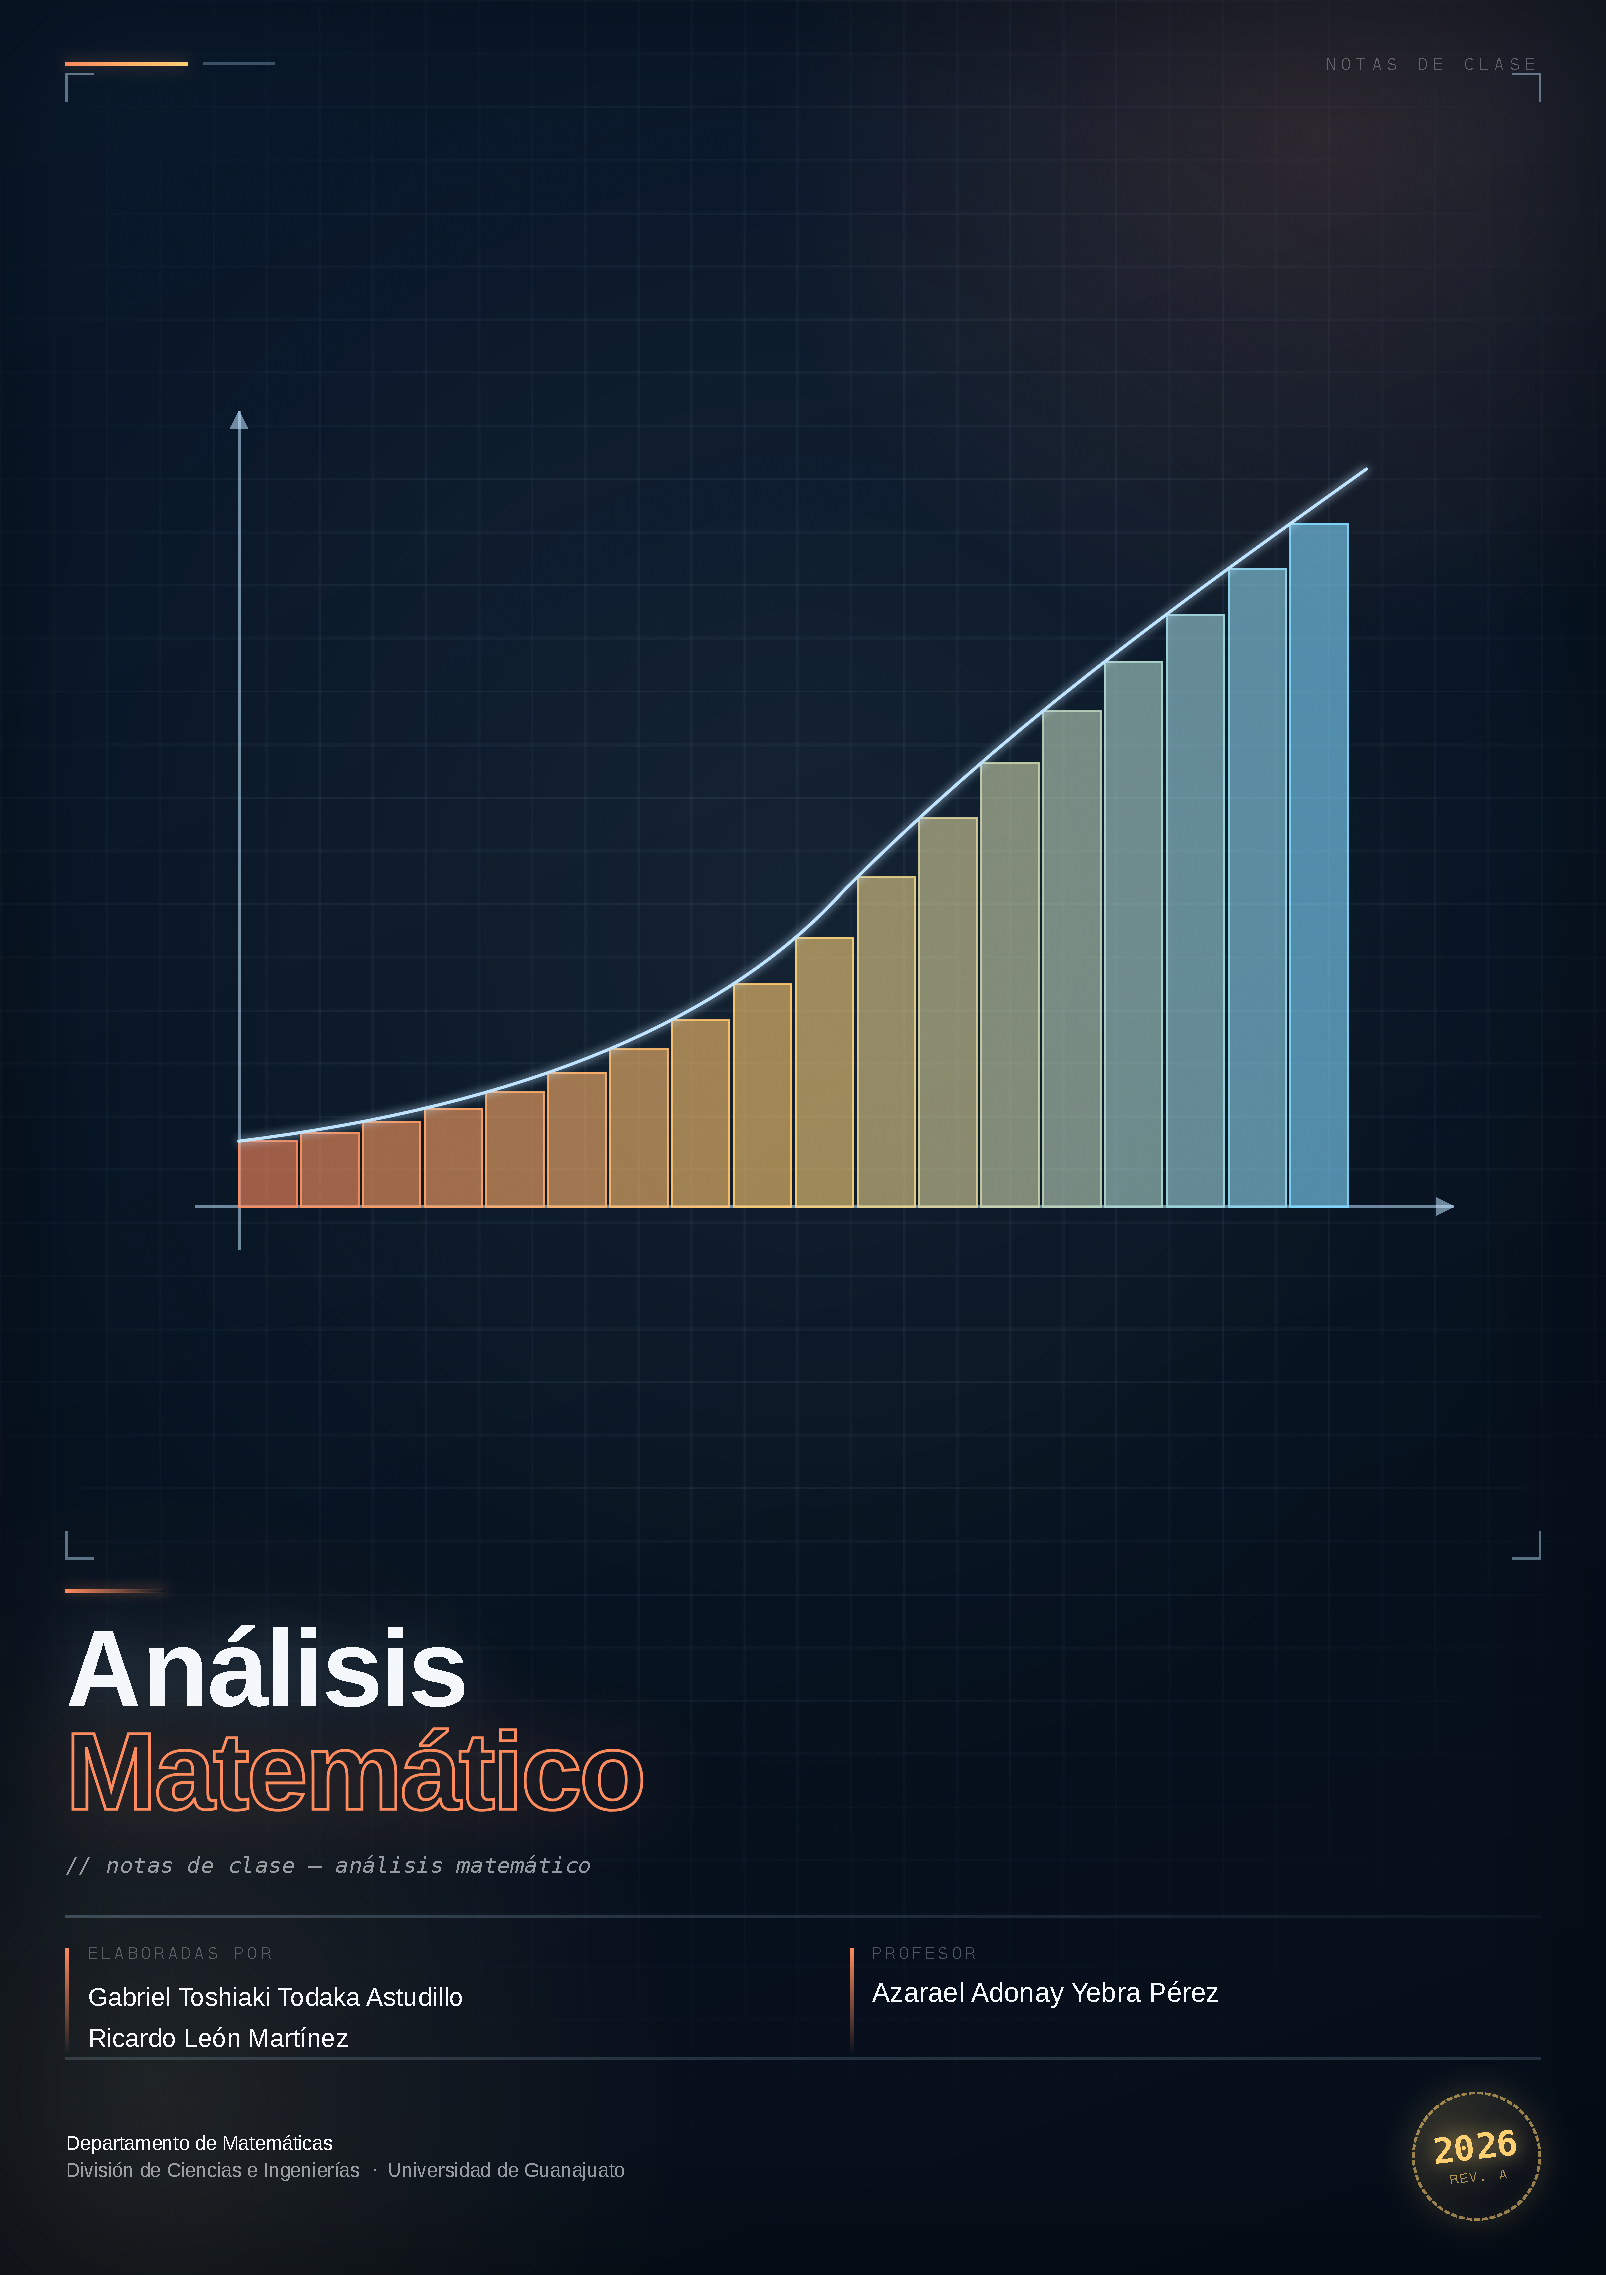
\includepdf[pages=1]{portada_analisis_matematico.pdf}

  \begin{flushright}
    \thispagestyle{empty}

    \textbf{Ricardo}\\[0.3cm]  
      Aqui son las dedicatorias pero hay que ponerlas hasta el final
      \textbf{Toshi}\\[0.3cm]
      Oka
  \end{flushright}

  % ---------------- NOTA DE ERRORES ----------------

  \cleardoublepage
  \thispagestyle{empty}

  \begin{mdframed}[style=mdgreenbox]
    \begin{center}
    \small
    Estas notas fueron elaboradas con fines académicos.\\
    A pesar del cuidado puesto en su redacción,\\
    es posible que existan errores u omisiones.\\[0.3cm]

    Cualquier corrección, sugerencia o comentario será bienvenido
    en los correos: \\[0.3cm]

    ricardo.leon@cimat.mx\\
    gt.todakaastudillo@ugto.mx
    \end{center}
  \end{mdframed}

  % -------------------------------------------------
    
  \setcounter{page}{1}
  \tableofcontents

  \chapter{El sistema de los números reales y complejos}
 
  En este capítulo construimos, a partir de un puñado de axiomas, el sistema de los números reales que usaremos durante todo el curso. Empezamos con el lenguaje básico de conjuntos, después presentamos los axiomas de cuerpo, de orden y de completitud que caracterizan a $\mathbb{R}$, y estudiamos a los números enteros: divisibilidad, inducción matemática y números primos. Al final construimos el sistema de los números complejos.
  
  % ======================================================
  \section{Notación básica de conjuntos}
  % ======================================================
  
  Para construir a los números reales necesitamos primero un poco del lenguaje básico de la teoría de conjuntos.
  
  \begin{definicion}[Conjunto]
    Un \textbf{conjunto} es una colección bien definida de objetos.
  \end{definicion}
  
  Por ejemplo, la colección de las vocales del abecedario, $\{a,e,i,o,u\}$, es un conjunto. Para indicar que $x$ es un elemento de un conjunto $A$ escribimos $x \in A$ (léase ``$x$ pertenece a $A$''), y para indicar que $x$ no es un elemento de $A$ escribimos $x \notin A$ (``$x$ no pertenece a $A$'').
  
  \begin{definicion}[Subconjunto]
    Diremos que un conjunto $A$ es \textbf{subconjunto} de un conjunto $B$, lo cual escribiremos $A \subset B$, si todo elemento de $A$ es también elemento de $B$.
  \end{definicion}
  
  Si $A \subset B$ pero $A \neq B$, decimos que $A$ es un \textbf{subconjunto propio} de $B$ y lo escribimos $A \subsetneq B$.

  Siempre que se introduce un objeto matemático hay que decir cuándo dos de esos objetos son iguales. Para conjuntos, el criterio es el siguiente.
  
  \noindent\textbf{Criterio (igualdad de conjuntos).} Dos conjuntos son iguales si y sólo si tienen exactamente los mismos elementos. En consecuencia, para probar que $A=B$ basta mostrar que $A \subset B$ y que $B \subset A$.
  
  \begin{definicion}[Conjunto vacío]
    El \textbf{conjunto vacío}, denotado por $\emptyset$, es el conjunto que no tiene elementos.
  \end{definicion}
  
  \begin{proposicion}
    El conjunto vacío es subconjunto de cualquier conjunto.
  \end{proposicion}
  
  \begin{proof}
    Procedemos por contradicción. Supongamos que existe un conjunto $A$ tal que $\emptyset \not\subset A$. Esto significa que existe $x \in \emptyset$ con $x \notin A$, lo cual es imposible, pues el conjunto vacío no tiene elementos. Por lo tanto, tal conjunto $A$ no existe, y en consecuencia $\emptyset$ es subconjunto de cualquier conjunto.
  \end{proof}
  
  No todo conjunto se puede describir enumerando sus elementos entre llaves. Para estos casos usamos la \textbf{notación de conjuntos mediante una condición}: si $X$ es un conjunto y $P(x)$ es una condición sobre los elementos de $X$, escribimos
  \begin{equation*}
    \{x \in X : P(x)\}
  \end{equation*}
  para denotar al conjunto de los $x \in X$ tales que se cumple $P(x)$. El símbolo ``$:$'' se lee ``tal que'' (o ``tales que''). Cuando se trabaja con un conjunto fijo $X$, en ocasiones escribiremos simplemente $\{x : P(x)\}$, entendiendo que los $x$ en consideración son elementos de $X$.

  \begin{ejemplo}
    El conjunto de los reales positivos donde el seno se anula es
    \begin{equation*}
      S=\{x\in\mathbb{R} : \sin(x)=0 \text{ y } x>0\}=\{x : x=n\pi \text{ con } n\in\mathbb{N}\}=\{\pi,2\pi,3\pi,\dots\}.
    \end{equation*}
  \end{ejemplo}

  % ======================================================
  \section{Distintas clases de números}
  % ======================================================
  
  Recordemos que el conjunto de los números naturales es
  \begin{equation*}
    \mathbb{N} = \{1,2,3,4,\dots\}.
  \end{equation*}
  A partir de él definimos los enteros, los racionales y los irracionales:
  \begin{equation*}
    \mathbb{Z} = \{\dots,-3,-2,-1,0,1,2,3,\dots\}
  \end{equation*}
  \begin{equation*}
    \mathbb{Q} = \{a/b : a,b \in \mathbb{Z},\ b \neq 0\}
  \end{equation*}
  \begin{equation*}
    \mathbb{I} = \mathbb{R}\setminus\mathbb{Q}
  \end{equation*}
  es decir, el conjunto de los números irracionales es el conjunto de todos los números reales que no son racionales. Algunos irracionales conocidos son $\sqrt{2}$, $\pi$ y $e$. Notemos que
  \begin{equation*}
    \mathbb{N} \subset \mathbb{Z} \subset \mathbb{Q} \subset \mathbb{R}, \qquad \mathbb{I} \subset \mathbb{R}, \qquad \mathbb{R} = \mathbb{Q} \cup \mathbb{I}, \qquad \mathbb{Q} \cap \mathbb{I} = \emptyset.
  \end{equation*}
  
  Vale la pena notar que una misma fracción puede escribirse de más de una forma: $3/15$ y $1/5$ son expresiones distintas para el mismo número racional; cuando el numerador y el denominador no comparten factores comunes (como en $1/5$), decimos que la fracción está en su \textbf{forma reducida}.
  
  \begin{ejemplo}
    \textbf{Ejemplos de cada clase de número.}
    \begin{equation*}
      2\in\mathbb{N}, \qquad -3\in\mathbb{Z}\setminus\mathbb{N}, \qquad \frac{1}{2}\in\mathbb{Q}\setminus\mathbb{Z}, \qquad \sqrt{2},\ \pi,\ e \in\mathbb{I}.
    \end{equation*}
    Todo número racional tiene una expansión decimal finita o periódica; por ejemplo,
    \begin{equation*}
      \frac{1}{4}=0.25, \qquad \frac{1}{3}=0.\overline{3}=0.333\ldots
    \end{equation*}
    Los números irracionales, en cambio, tienen una expansión decimal infinita y no periódica; ésta es, de hecho, una manera equivalente de definir a $\mathbb{I}$.
  \end{ejemplo}
  
  % ======================================================
  \section{Axiomas de cuerpo}
  % ======================================================
  
  En $\mathbb{R}$ existen dos operaciones, la suma o adición ``$+$'' y el producto o multiplicación ``$\cdot$'', que satisfacen los axiomas siguientes. En lo que sigue, $x,y,z$ denotan números reales.
  
  \begin{enumerate}[leftmargin=2.4em]
    \item[\textbf{1.}] \textbf{Conmutatividad de la suma:} $x+y=y+x$.
    \item[\textbf{2.}] \textbf{Asociatividad de la suma:} $x+(y+z)=(x+y)+z$.
    \item[\textbf{3.}] \textbf{Existencia del neutro aditivo:} existe un número real, denotado por $0$, tal que $x+0=x$.
    \item[\textbf{4.}] \textbf{Existencia de inversos aditivos:} dado $x \in \mathbb{R}$, existe un número real, llamado el inverso aditivo de $x$ y denotado por $-x$, tal que $x+(-x)=0$.
    \item[\textbf{5.}] \textbf{Conmutatividad del producto:} $x\cdot y = y \cdot x$.
    \item[\textbf{6.}] \textbf{Asociatividad del producto:} $x\cdot(y\cdot z)=(x\cdot y)\cdot z$.
    \item[\textbf{7.}] \textbf{Existencia del neutro multiplicativo:} existe un número real distinto de $0$, denotado por $1$, tal que $x \cdot 1 = x$.
    \item[\textbf{8.}] \textbf{Existencia de inversos multiplicativos:} dado $x \in \mathbb{R}$ con $x \neq 0$, existe un número real, llamado el inverso multiplicativo de $x$ y denotado por $x^{-1}$, tal que $x \cdot x^{-1}=1$.
    \item[\textbf{9.}] \textbf{Distributividad:} $x\cdot(y+z) = x\cdot y + x\cdot z$.
  \end{enumerate}
  
  Notemos que los primeros cuatro axiomas se refieren a la suma, los cuatro siguientes al producto, y el último relaciona ambas operaciones. Otros símbolos que usaremos para el producto $x\cdot y$ son $xy$, $x(y)$ y $(x)(y)$.
  
  De estos nueve axiomas se sigue, usando la asociatividad, que la suma (o el producto) de tres o más números reales no depende de cómo los agrupemos; por ello escribimos simplemente $x+y+z$ o $xyz$ sin paréntesis.
  
  Con los axiomas 4 y 8 podemos definir la resta y la división.
  
  \begin{definicion}[Resta y división de números reales]
    Sean $x,y \in \mathbb{R}$.
    \begin{enumerate}[label=(\alph*)]
      \item Definimos la \textbf{resta} de $x$ menos $y$ como $x-y = x+(-y)$.
      \item Si $x \neq 0$, definimos el \textbf{cociente} de $y$ entre $x$ como $\dfrac{y}{x} = y \cdot x^{-1}$.
    \end{enumerate}
  \end{definicion}
  
  Un primer resultado de los axiomas de cuerpo son las leyes de cancelación, que hemos usado desde nuestros cursos de álgebra elemental para ``despejar'' una variable en una ecuación.
  
  \begin{proposicion}[Leyes de cancelación]
    \begin{enumerate}[label=(\alph*)]
      \item Si $x+y=z$, entonces $y=z-x$.
      \item Si $x \neq 0$ y $xy=z$, entonces $y = z/x$.
    \end{enumerate}
  \end{proposicion}
  
  \begin{proof}
    (a) Notemos que
    \begin{align*}
      x+y                  & =z                                                \\
      \Rightarrow -x+(x+y) & = -x+z   &  & \text{(sumamos $-x$ a ambos lados)} \\
      \Rightarrow (-x+x)+y & = -x+z   &  & \text{(asociatividad de la suma)}   \\
      \Rightarrow 0+y      & = -x+z   &  & \text{(propiedad de $-x$)}          \\
      \Rightarrow y        & = -x+z   &  & \text{(propiedad del $0$)}          \\
      \Rightarrow y        & = z+(-x) &  & \text{(conmutatividad de la suma)}  \\
      \Rightarrow y        & = z-x.   &  & \text{(definición de la resta)}
    \end{align*}
    La demostración del inciso (b) es análoga, usando el axioma 8 en vez del axioma 4.
  \end{proof}
  
  Con la ley de cancelación podemos mostrar que los inversos aditivo y multiplicativo de un número son únicos.
  
  \begin{proposicion}[Unicidad de los inversos]
    \begin{enumerate}[label=(\alph*)]
      \item Dado $x \in \mathbb{R}$, el número $-x$ es el único real que satisface $x+(-x)=0$.
      \item Dado $x \in \mathbb{R}$ con $x \neq 0$, el número $x^{-1}$ es el único real que satisface $x \cdot x^{-1}=1$.
    \end{enumerate}
  \end{proposicion}
  
  \begin{proof}
    (a) Supongamos que $y$ satisface $x+y=0$. Por la ley de cancelación (con $z=0$), $y=0-x=-x$. La demostración de (b) es análoga.
  \end{proof}
  
  \begin{corolario}
    Para todo $x \in \mathbb{R}$ se cumple que $-(-x)=x$.
  \end{corolario}
  
  \begin{proof}
    Por el axioma 4, $(-x)+x=0$, es decir, $x$ satisface la ecuación que define al inverso aditivo de $-x$. Por la unicidad de los inversos, $x$ debe ser precisamente ese inverso, es decir, $x=-(-x)$.
  \end{proof}
  
  % ======================================================
  \section{Axiomas de orden}
  % ======================================================
  
  Además de la suma y el producto, en $\mathbb{R}$ contamos con una relación de orden ``$<$'' entre números reales que cumple los axiomas siguientes (la expresión $x<y$ se lee ``$x$ es menor que $y$''; geométricamente, significa que al situar a $x$ y a $y$ sobre la recta numérica, $x$ queda a la izquierda de $y$).
  
  \begin{enumerate}[leftmargin=2.6em]
    \item[\textbf{10.}] \textbf{Tricotomía:} dados $x,y \in \mathbb{R}$, se cumple una y sólo una de las condiciones
          \begin{equation*}
            x<y, \qquad x=y, \qquad y<x.
          \end{equation*}
    \item[\textbf{11.}] \textbf{Transitividad:} si $x<y$ y $y<z$, entonces $x<z$.
    \item[\textbf{12.}] \textbf{Preservación del orden bajo la suma:} si $x<y$, entonces $x+z<y+z$ para todo $z \in \mathbb{R}$.
    \item[\textbf{13.}] \textbf{Preservación del orden bajo el producto por positivos:} si $x<y$ y $z$ es positivo, entonces $xz<yz$.
  \end{enumerate}
  
  Antes de seguir necesitamos precisar qué significa que un número sea positivo o negativo.
  
  \begin{definicion}[Números positivos y negativos]
    Sea $x \in \mathbb{R}$.
    \begin{enumerate}[label=(\alph*)]
      \item Diremos que $x$ es \textbf{positivo} si $0<x$.
      \item Diremos que $x$ es \textbf{negativo} si $x<0$.
    \end{enumerate}
  \end{definicion}
  
  Además de ``$<$'', definimos las relaciones siguientes.
  
  \begin{definicion}
    Sean $x,y \in \mathbb{R}$.
    \begin{enumerate}[label=(\alph*)]
      \item Definimos $x>y$ si $y<x$.
      \item Definimos $x \leq y$ si $x<y$ o $x=y$.
      \item Definimos $x \geq y$ si $y \leq x$.
    \end{enumerate}
  \end{definicion}
  
  La primera consecuencia de los axiomas de orden es la siguiente.
  
  \begin{proposicion}
    Sean $x,y \in \mathbb{R}$. Entonces $x<y$ si y sólo si $y-x>0$.
  \end{proposicion}
  
  \begin{proof}
    Por la preservación del orden bajo la suma (axioma 12),
    \begin{equation*}
      x<y \;\Rightarrow\; x-x < y-x \;\Rightarrow\; 0<y-x \quad \text{(por la propiedad de $-x$).}
    \end{equation*}
    Las implicaciones contrarias también se cumplen (basta sumar $x$ a ambos lados), de donde se sigue la equivalencia.
  \end{proof}
  
  También necesitaremos la siguiente propiedad, útil para acotar un número por otro salvo un error arbitrariamente pequeño.
  
  \begin{proposicion}
    Si $a,b \in \mathbb{R}$ satisfacen $a \leq b+\varepsilon$ para todo $\varepsilon>0$, entonces $a \leq b$.
  \end{proposicion}
  
  \begin{proof}
    Procedemos por contradicción. Supongamos que $b<a$, y tomemos $\varepsilon = \dfrac{a-b}{2}>0$ (positivo, pues $a>b$ por la proposición anterior). Notemos que
    \begin{equation*}
      b+\varepsilon = b+\frac{a-b}{2} = \frac{a+b}{2}.
    \end{equation*}
    Por otro lado, de $b<a$ y el axioma 12,
    \begin{equation*}
      b<a \;\Rightarrow\; b+a<a+a=2a \;\Rightarrow\; \frac{a+b}{2}<a.
    \end{equation*}
    Así, $b+\varepsilon<a$, es decir, $a>b+\varepsilon$, lo cual contradice la hipótesis $a\leq b+\varepsilon$ para ese mismo $\varepsilon$. Por lo tanto $b<a$ es imposible, y concluimos que $a \leq b$.
  \end{proof}
  
  % ======================================================
  \section{Cotas, supremo e ínfimo}
  % ======================================================
  
  Los axiomas de orden nos permiten comparar dos números reales a la vez. Ahora usaremos ese orden para describir el comportamiento de un \emph{conjunto completo} de números reales: qué tan ``grande'' o ``pequeño'' puede llegar a ser.
  
  \begin{definicion}[Cota superior]
    Sea $S$ un conjunto de números reales. Si existe un número real $b$ tal que $x\leq b$ para todo $x\in S$, diremos que $b$ es una \textbf{cota superior} de $S$ y que $S$ está \textbf{acotado superiormente} por $b$.
  
    Si $b$ es cota superior de $S$ y además $b\in S$, entonces lo denominamos el \textbf{máximo} de $S$, y lo denotamos por $b=\max S$.
  \end{definicion}
  
  Los conjuntos sin cotas superiores se llaman \textbf{no acotados superiormente}.
  
  \begin{definicion}[Cota inferior]
    Sea $S$ un conjunto de números reales. Si existe un número real $a$ tal que $a\leq x$ para todo $x\in S$, diremos que $a$ es una \textbf{cota inferior} de $S$ y que $S$ está \textbf{acotado inferiormente} por $a$.
  
    Si $a$ es cota inferior de $S$ y además $a\in S$, entonces lo denominamos el \textbf{mínimo} de $S$, y lo denotamos por $a=\min S$.
  \end{definicion}
  
  \begin{ejemplo}
    \textbf{Cotas superiores e inferiores.}
    \begin{enumerate}[label=(\arabic*)]
      \item $\mathbb{R}=(-\infty,\infty)$ no tiene cota inferior ni cota superior.
      \item $\mathbb{R}^+=(0,\infty)$: $0$ es una cota inferior, pero $\mathbb{R}^+$ no tiene cota superior. Además, $\mathbb{R}^+$ carece de mínimo, pues $0\notin\mathbb{R}^+$.
      \item $\mathbb{R}^+\cup\{0\}=[0,\infty)$: $0$ es una cota inferior y el conjunto no está acotado superiormente. Como $0$ pertenece al conjunto, $\min(\mathbb{R}^+\cup\{0\})=0$.
      \item $S=[0,2]$ es un conjunto acotado: $0$ es una cota inferior y $2$ es una cota superior, con $\min S=0$ y $\max S=2$.
      \item $T=[1,3)$ está acotado inferior y superiormente, con $\min T=1$; sin embargo, $\max T$ no existe (ningún elemento de $T$ es mayor o igual que todos los demás, pues $T$ no incluye a su extremo derecho).
    \end{enumerate}
  \end{ejemplo}
  
  El último ejemplo muestra que un conjunto acotado superiormente no siempre tiene máximo. Sin embargo, entre todas las cotas superiores de un conjunto acotado siempre hay una que es la ``mejor'' posible: la más pequeña. A esa cota especial la llamamos el \textbf{supremo}.
  
  \begin{definicion}[Supremo]
    Sea $S$ un conjunto de números reales acotado superiormente. Un número real $b$ se denomina \textbf{extremo superior} o \textbf{supremo} de $S$ si satisface las dos propiedades siguientes:
    \begin{enumerate}[label=(\arabic*)]
      \item $b$ es una cota superior de $S$.
      \item Ningún número menor que $b$ es cota superior de $S$.
    \end{enumerate}
    Al número $b$ que satisface ambas propiedades lo denotamos por $b=\sup S$.
  \end{definicion}
  
  En otras palabras, el supremo es la cota superior más pequeña.
  
  \begin{definicion}[Ínfimo]
    Sea $S$ un conjunto de números reales acotado inferiormente. Un número real $a$ se denomina \textbf{extremo inferior} o \textbf{ínfimo} de $S$ si satisface las dos propiedades siguientes:
    \begin{enumerate}[label=(\arabic*)]
      \item $a$ es una cota inferior de $S$.
      \item Ningún número mayor que $a$ es cota inferior de $S$.
    \end{enumerate}
    Al número $a$ que satisface ambas propiedades lo representamos por $a=\inf S$.
  \end{definicion}
  
  Análogamente, el ínfimo es la cota inferior más grande. Cuando el máximo (o el mínimo) de un conjunto existe, coincide con su supremo (o su ínfimo, respectivamente); pero, como muestra el siguiente ejemplo, el supremo y el ínfimo pueden existir incluso cuando el máximo o el mínimo no.
  
  \begin{ejemplo}
    \textbf{Supremo e ínfimo.}
    \begin{enumerate}[label=(\arabic*)]
      \item $S=[0,1]$: está acotado por sus extremos. Como $0\in S$, $\min S = \inf S = 0$; y como $1\in S$, $\max S = \sup S = 1$.
      \item $T=[0,1)$: $0$ es cota inferior y $0\in T$, así que $\min T = \inf T = 0$. Por otro lado, $1$ es cota superior de $T$, pero no existe $\max T$ (pues $1\notin T$); sin embargo, ninguna cota superior menor que $1$ funciona (siempre hay elementos de $T$ más grandes que ella), así que $\sup T = 1$.
    \end{enumerate}
  \end{ejemplo}
  
  Hasta ahora, nada en los axiomas de cuerpo y de orden garantiza que un conjunto acotado superiormente efectivamente \emph{tenga} un supremo (de hecho, $\mathbb{Q}$ satisface ambos tipos de axiomas y, sin embargo, el conjunto $\{x\in\mathbb{Q} : x^2<2\}$, acotado superiormente en $\mathbb{Q}$, no tiene supremo racional). Por ello necesitamos un último axioma, que es precisamente lo que distingue a $\mathbb{R}$ de $\mathbb{Q}$.
  
  \noindent\textbf{Axioma (completitud, o axioma del supremo).} Se cumplen las dos afirmaciones siguientes:
  \begin{enumerate}[label=(\alph*)]
    \item Todo conjunto no vacío $S$ de números reales que esté acotado superiormente admite un supremo; es decir, existe un número real $b$ tal que $b=\sup S$.
    \item Todo conjunto no vacío $S$ de números reales que esté acotado inferiormente admite un ínfimo; es decir, existe un número real $a$ tal que $a=\inf S$.
  \end{enumerate}
  
  El axioma de completitud es, junto con los axiomas de cuerpo y de orden, uno de los tres pilares sobre los que se construye $\mathbb{R}$: cualquier conjunto de números que satisfaga los tres tipos de axiomas es, esencialmente, una copia de los números reales.
  
  % ======================================================
  \section{El número \texorpdfstring{$e$}{e} es irracional}
  % ======================================================
  
  Como aplicación de las herramientas anteriores, mostramos que el número $e$, definido mediante la serie
  \begin{equation*}
    e = \sum_{k=0}^{\infty} \frac{1}{k!} = 1+1+\frac{1}{2!}+\frac{1}{3!}+\cdots,
  \end{equation*}
  no es racional. La demostración combina un argumento de divisibilidad (¿qué tan bien se puede aproximar $e$ por una suma finita?) con una cota tipo serie geométrica.
  
  \begin{teorema}[Irracionalidad de $e$]
    El número $e$ es irracional.
  \end{teorema}
  
  \begin{proof}
    Procedemos por contradicción. Supongamos que $e$ es racional, es decir, $e=\dfrac{a}{b}$ para ciertos $a,b\in\mathbb{Z}^+$. Multiplicando por $b!$,
    \begin{equation*}
      b!\,e = a(b-1)!,
    \end{equation*}
    que es un entero positivo.
  
    Por otro lado, usando la serie que define a $e$,
    \begin{equation*}
      b!\,e = b!\sum_{k=0}^{\infty}\frac{1}{k!} = \sum_{k=0}^{\infty}\frac{b!}{k!} = \underbrace{\sum_{k=0}^{b}\frac{b!}{k!}}_{(\ast)} + \underbrace{\sum_{k=b+1}^{\infty}\frac{b!}{k!}}_{(\ast\ast)}.
    \end{equation*}
  
    \textbf{La suma $(\ast)$ es un entero positivo:} para $0\leq k\leq b$, el cociente $\dfrac{b!}{k!}=(k+1)(k+2)\cdots b$ es un producto de enteros, así que cada término (y por lo tanto la suma completa) es un entero positivo.
  
    \textbf{La suma $(\ast\ast)$ está estrictamente entre $0$ y $1$:} escribiendo $k=b+i$ con $i\geq 1$,
    \begin{equation*}
      (\ast\ast) = \sum_{i=1}^{\infty}\frac{b!}{(b+i)!} = \sum_{i=1}^{\infty}\frac{1}{(b+1)(b+2)\cdots(b+i)}.
    \end{equation*}
    Como $b+1<b+2<\cdots<b+i$, se tiene $(b+1)(b+2)\cdots(b+i) \geq (b+1)^i$, así que
    \begin{equation*}
      0 < (\ast\ast) \leq \sum_{i=1}^{\infty}\frac{1}{(b+1)^i}.
    \end{equation*}
    Esta última es una serie geométrica de razón $r=\dfrac{1}{b+1}<1$ (pues $b\geq 1$), así que
    \begin{equation*}
      \sum_{i=1}^{\infty}\frac{1}{(b+1)^i} = \frac{\frac{1}{b+1}}{1-\frac{1}{b+1}} = \frac{1}{b} \leq 1.
    \end{equation*}
    Por lo tanto, $0<(\ast\ast)<1$ (la desigualdad es estricta pues $(b+1)(b+2)\cdots(b+i)>(b+1)^i$ para $i\geq 2$).
  
    \textbf{Conclusión.} Hemos mostrado que
    \begin{equation*}
      b!\,e = \underbrace{(\ast)}_{\in\,\mathbb{Z}^+} + \underbrace{(\ast\ast)}_{0<\,\cdot\,<1},
    \end{equation*}
    pero también que $b!\,e = a(b-1)!\in\mathbb{Z}^+$. Como no existe ningún entero estrictamente entre $0$ y $1$, un entero no puede escribirse como otro entero más una cantidad estrictamente entre $0$ y $1$. Esta contradicción muestra que la suposición inicial es falsa. Por lo tanto, $e$ no puede ser racional.
  \end{proof}
  
  \begin{problema}
    Demostrar, con un argumento similar, que $\pi$ es irracional.
  \end{problema}
  
  % ======================================================
  \section{Representación geométrica e intervalos}
  % ======================================================
  
  Cada número real se representa como un punto sobre una recta, la \emph{recta real o recta numérica}. Las relaciones ``$<$'' y ``$\leq$'' permiten definir un tipo especial de subconjuntos de $\mathbb{R}$ a los que llamaremos \textbf{intervalos}.
  
  \begin{definicion}[Intervalos]
    Sean $a,b \in \mathbb{R}$.
    \begin{enumerate}[label=(\alph*)]
      \item Definimos los intervalos finitos
            \begin{equation*}
              (a,b) = \{x : a<x<b\}, \qquad [a,b] = \{x : a \leq x \leq b\},
            \end{equation*}
            \begin{equation*}
              (a,b] = \{x : a<x\leq b\}, \qquad [a,b) = \{x : a \leq x <b\}.
            \end{equation*}
            Al conjunto $(a,b)$ le llamamos \textbf{intervalo abierto}, a $[a,b]$ \textbf{intervalo cerrado}, a $(a,b]$ \textbf{intervalo semiabierto por la izquierda y semicerrado por la derecha}, y a $[a,b)$ \textbf{intervalo semicerrado por la izquierda y semiabierto por la derecha}.
      \item Definimos también los intervalos infinitos
            \begin{equation*}
              (a,\infty) = \{x : a<x\}, \quad [a,\infty) = \{x : a \leq x\}, \quad (-\infty,a) = \{x : x<a\},
            \end{equation*}
            \begin{equation*}
              (-\infty,a] = \{x : x \leq a\}, \qquad (-\infty,\infty) = \mathbb{R}.
            \end{equation*}
    \end{enumerate}
  \end{definicion}
  
  Notemos que si $b<a$, entonces $(a,b)=[a,b]=(a,b]=[a,b)=\emptyset$; también $(a,a)=(a,a]=[a,a)=\emptyset$, mientras que $[a,a]=\{a\}$. De aquí en adelante, salvo que se indique lo contrario, al considerar intervalos de la forma $(a,b)$, $(a,b]$ o $[a,b)$ supondremos que $a<b$, y al considerar $[a,b]$ supondremos que $a \leq b$.
  
  % ======================================================
  \section{Conjuntos inductivos y los números enteros}
  % ======================================================
  
  Para caracterizar con precisión al conjunto de los números enteros (y más adelante a los números primos) usamos la noción de \textbf{conjunto inductivo}.
  
  \begin{definicion}[Conjunto inductivo]
    Un conjunto de números reales se denomina \textbf{conjunto inductivo} si:
    \begin{enumerate}[label=(\alph*)]
      \item $1$ pertenece al conjunto.
      \item Para cada $x$ del conjunto, el número $x+1$ también pertenece al conjunto.
    \end{enumerate}
  \end{definicion}
  
  Es decir, un conjunto inductivo empieza en $1$ y, una vez dentro, no es posible ``salir'' sumando $1$ repetidamente; esto es justamente lo que hace a $\mathbb{N}=\{1,2,3,\dots\}$ un conjunto inductivo.
  
  \begin{definicion}[Entero]
    Un número real se denomina \textbf{entero} si pertenece a todo conjunto inductivo. El conjunto de los enteros positivos se designa por $\mathbb{Z}^+$.
  \end{definicion}
  
  $\mathbb{Z}^+$ es el menor conjunto inductivo, en el sentido de que está contenido en cualquier otro. A los inversos aditivos de los enteros positivos los llamamos \textbf{enteros negativos}, $\mathbb{Z}^-$. Así,
  \begin{equation*}
    \mathbb{Z}^+ \cup \mathbb{Z}^- \cup \{0\} = \mathbb{Z} \quad \Longrightarrow \quad (\mathbb{Z},+) \text{ es un grupo.}
  \end{equation*}
  
  \subsection{Divisibilidad: definiciones básicas}
  
  \begin{definicion}[Divisor y múltiplo]
    Sean $a,d \in \mathbb{Z}$. Diremos que $d$ \textbf{divide} a $a$, lo cual escribimos $d \mid a$, si existe un entero $c$ tal que $a=cd$. En este caso decimos que $d$ es un \textbf{divisor} o \textbf{factor} de $a$, y que $a$ es un \textbf{múltiplo} de $d$.
  \end{definicion}
  
  \begin{ejemplo}
    $3\mid 12$, pues $12=4\cdot 3$; los divisores positivos de $12$ son $1,2,3,4,6,12$. En cambio, $3\nmid 7$: no existe ningún entero $c$ tal que $7=3c$.
  \end{ejemplo}
  
  \begin{definicion}[Número primo]
    Un \textbf{número primo} es un número natural mayor que $1$ cuyos únicos divisores positivos son él mismo y la unidad.
  \end{definicion}
  
  \begin{definicion}[Número compuesto]
    Si $n>0$ y $n$ no es primo ni es $1$, decimos que $n$ es \textbf{compuesto}.
  \end{definicion}
  
  \begin{ejemplo}
    Los primeros números primos son
    \begin{equation*}
      2,3,5,7,11,13,17,19,23,29,\dots
    \end{equation*}
    Notemos que $2$ es el único primo par: cualquier otro número par $n=2k$ con $k>1$ tiene a $2$ como divisor propio, así que es compuesto. Los primeros números compuestos son $4,6,8,9,10,12,\dots$; el número $1$ no se considera ni primo ni compuesto.
  \end{ejemplo}
  
  Si $d$ no divide a $a$ escribimos $d \nmid a$.
  
  % ======================================================
  \section{Principio de inducción}
  % ======================================================
  
  En esta sección estudiamos el \textbf{principio de inducción matemática}, una herramienta fundamental para probar afirmaciones de la forma $\forall n \in \mathbb{N},\ P(n)$.
  
  \begin{proposicion}[Principio de inducción matemática]
    Sea $A \subset \mathbb{N}$. Supongamos que $A$ cumple las dos condiciones siguientes:
    \begin{enumerate}[label=(\alph*)]
      \item $1 \in A$.
      \item Si $k \in A$, entonces $k+1 \in A$.
    \end{enumerate}
    Entonces $A=\mathbb{N}$.
  \end{proposicion}
  
  A la hipótesis del inciso (b) se le conoce como \textbf{hipótesis de inducción}. El principio se usa para probar que una fórmula o condición $P(n)$ se cumple para todo $n \in \mathbb{N}$: basta considerar el conjunto $A=\{n \in \mathbb{N} : P(n) \text{ se cumple}\}$ y verificar que cumple (a) y (b); entonces $A=\mathbb{N}$, es decir, $P(n)$ se cumple para todo $n$.
  
  \begin{ejemplo}
    \textbf{Suma de los primeros $n$ enteros.}
    Probemos que para todo $n \in \mathbb{N}$ se cumple que
    \begin{equation*}
      1+2+\cdots+n = \frac{n(n+1)}{2}.
    \end{equation*}
  
    \textbf{Solución.} Sea $P(n)$ la fórmula anterior y consideremos $A=\{n \in \mathbb{N} : P(n)\}$. Mostraremos que $A$ cumple las condiciones (a) y (b) del principio de inducción.
  
    (a) Es claro que $1 \in A$, pues $1 = 1(1+1)/2$.
  
    (b) Supongamos que $k \in A$, es decir, que $1+2+\cdots+k = k(k+1)/2$. Entonces
    \begin{equation*}
      1+2+\cdots+k+(k+1) = \frac{k(k+1)}{2}+(k+1) = \frac{k(k+1)+2(k+1)}{2} = \frac{(k+1)(k+2)}{2},
    \end{equation*}
    lo cual muestra que $k+1 \in A$.
  
    Por el principio de inducción, $A=\mathbb{N}$, es decir, la fórmula se cumple para todo $n \in \mathbb{N}$.
  \end{ejemplo}
  
  En la práctica, la prueba de que $P(n)$ se cumple para todo $n$, como la del ejemplo anterior, se abrevia probando sólo lo siguiente:
  \begin{enumerate}[label=(\roman*)]
    \item $P(n)$ se cumple para $n=1$ (\emph{base inductiva}).
    \item Si $P(n)$ se cumple para $n=k$, entonces se cumple para $n=k+1$ (\emph{paso inductivo}).
  \end{enumerate}
  
  \begin{problema}
    Demostrar por inducción la siguiente fórmula:
    \begin{equation*}
      1^2+2^2+3^2+\cdots+n^2 = \frac{n(n+1)(2n+1)}{6}
    \end{equation*}
  \end{problema}
  
  % ======================================================
  \section{Propiedades de divisibilidad}
  % ======================================================
  
  Sean $a,b,c,d,n,m \in \mathbb{Z}$. La divisibilidad satisface las siguientes propiedades:
  
  \begin{center}
    \begin{tabular}{lll}
      \toprule
            & \textbf{Propiedad} & \textbf{Enunciado}                                  \\
      \midrule
      i)    & Reflexiva          & $n \mid n$                                          \\
      ii)   & Transitiva         & $d\mid n$ y $n\mid m$ $\Rightarrow$ $d\mid m$       \\
      iii)  & Linealidad         & $d\mid n$ y $d\mid m$ $\Rightarrow$ $d\mid (an+bm)$ \\
      iv)   & Multiplicación     & $d\mid n$ $\Rightarrow$ $ad\mid an$                 \\
      v)    & Cancelación        & $ad\mid an$ y $a\neq 0$ $\Rightarrow$ $d\mid n$     \\
      vi)   & Unidad             & $1\mid n$ \quad (1 divide a cualquier entero)       \\
      vii)  & Cero               & $n\mid 0$ \quad (todo entero divide a 0)            \\
      viii) & Comparación        & $d\mid n$ y $n\neq 0$ $\Rightarrow$ $|d|\leq |n|$   \\
      ix)   & Antisimetría       & $d\mid n$ y $n\mid d$ $\Rightarrow$ $|d|=|n|$       \\
      x)    & Divisor conjugado  & $d\mid n$ y $d\neq 0$ $\Rightarrow$ $(n/d)\mid n$   \\
      xi)   & Sólo el cero       & $0\mid n$ $\Rightarrow$ $n=0$                       \\
      \bottomrule
    \end{tabular}
  \end{center}
  
  \begin{definicion}[Divisor conjugado]
    Si $d\mid n$, al número $n/d$ se le llama \textbf{divisor conjugado} de $d$.
  \end{definicion}
  
  \begin{definicion}[Común divisor]
    Si $d\mid a$ y $d\mid b$, decimos que $d$ es \textbf{común divisor} de $a$ y $b$. El $1$ siempre es un común divisor de cualquier par de enteros.
  \end{definicion}
  
  \begin{ejemplo}
    \textbf{Propiedades de divisibilidad en acción.}
    \begin{itemize}
      \item \textbf{Transitiva:} $3\mid 12$ y $12\mid 24$, así que $3\mid 24$.
      \item \textbf{Linealidad:} $4\mid 8$ y $4\mid 20$, así que $4\mid(3\cdot 8+2\cdot 20)=4\mid 76$ (en efecto, $76=19\cdot 4$).
      \item \textbf{Divisor conjugado:} como $3\mid 12$, el divisor conjugado de $3$ es $12/3=4$; y en efecto $4$ también divide a $12$.
      \item \textbf{Común divisor:} los divisores positivos de $12$ son $1,2,3,4,6,12$, y los de $20$ son $1,2,4,5,10,20$; los comunes son $1,2,4$, así que $4$ es el mayor de ellos.
    \end{itemize}
  \end{ejemplo}
  
  \begin{teorema}[Existencia de un común divisor como combinación lineal]
    Dados dos números $a$ y $b$, existe un común divisor $d$ de ambos que puede escribirse en la forma
    \begin{equation*}
      d = xa+yb, \qquad x,y \in \mathbb{Z}.
    \end{equation*}
    Además, cada divisor común de $a$ y $b$ divide a $d$.
  \end{teorema}
  
  \begin{teorema}[Todo entero mayor que 1 se factoriza en primos]
    Cada número entero $n>1$ es primo, o bien producto de números primos.
  \end{teorema}
  
  \begin{proof}
    Por inducción (fuerte).
  
    \textbf{Base inductiva:}
    \begin{equation*}
      n=2=1\cdot 2, \qquad n=3=1\cdot 3, \qquad n=4=2\cdot 2.
    \end{equation*}
  
    \textbf{Hipótesis.} El teorema se cumple para todo entero $k$ con $1<k<n$.
  
    \textbf{Paso inductivo.} Consideramos $k+1$. Si $k+1$ es primo, no hay nada más que probar. Si $k+1$ no es primo, entonces $k+1=cd$ con $1<c\leq k$ y $1<d\leq k$. Por la hipótesis de inducción, tanto $c$ como $d$ son primos o producto de primos, y por lo tanto también lo es $k+1=cd$.
  \end{proof}
  
  \begin{teorema}[Existencia y unicidad del máximo común divisor]
    Dados los enteros $a$ y $b$, existe un único $d$ con las siguientes propiedades:
    \begin{enumerate}[label=\roman*)]
      \item $d \geq 0$,
      \item $d\mid a$ y $d\mid b$ ($d$ es divisor común),
      \item si $e\mid a$ y $e\mid b$, entonces $e\mid d$ (todo divisor común de $a,b$ divide a $d$).
    \end{enumerate}
  \end{teorema}
  
  \begin{definicion}[Máximo común divisor (mcd)]
    El número $d$ del teorema anterior se llama \textbf{máximo común divisor} de $a$ y $b$, y se denota $d=(a,b)$ o $d=\gcd(a,b)$.
  \end{definicion}
  
  \begin{definicion}[Números coprimos]
    Si $(a,b)=1$, decimos que $a$ y $b$ son \textbf{primos entre sí} (o \textbf{coprimos}).
  \end{definicion}
  
  \begin{ejemplo}
    \textbf{Cálculo del mcd por listado de divisores.}
    Retomando el ejemplo anterior, los divisores positivos comunes de $12$ y $20$ son $1,2,4$; el mayor de ellos es $4$, así que $(12,20)=4$. Este método funciona bien para números pequeños, pero se vuelve poco práctico para números grandes; en un curso de teoría de números se estudia el \textbf{algoritmo de Euclides}, un método mucho más eficiente para calcular el mcd de cualquier par de enteros.
  \end{ejemplo}
  
  \begin{ejemplo}
    \begin{equation*}
      7=1\cdot 7, \qquad 13=1\cdot 13, \qquad 35=5\cdot 7
    \end{equation*}
    \begin{equation*}
      11=1\cdot 11, \qquad 6=1\cdot 2\cdot 3, \qquad 66=1\cdot 2\cdot 3\cdot 11
    \end{equation*}
    Como estas factorizaciones no comparten factores primos:
    \begin{equation*}
      (7,11)=1, \qquad (13,6)=1, \qquad (35,66)=1 \;\Longrightarrow\; 35 \text{ y } 66 \text{ son coprimos.}
    \end{equation*}
  \end{ejemplo}
  
  \begin{teorema}[Propiedades del mcd]
    \begin{enumerate}[label=\roman*)]
      \item \textbf{Conmutativa:} $(a,b)=(b,a)$
      \item \textbf{Asociativa:} $(a,(b,c)) = ((a,b),c)$
      \item \textbf{Distributiva:} $(ac,bc) = |c|\,(a,b)$
      \item \textbf{Casos base:} $(a,1)=(1,a)=1$, \qquad $(a,0)=(0,a)=|a|$
    \end{enumerate}
  \end{teorema}
  
  \begin{lema}[Lema de Euclides]
    Si $a\mid bc$ y $(a,b)=1$, entonces $a\mid c$.
  \end{lema}
  
  En palabras: si $a$ divide a un producto $bc$, pero $a$ no comparte factores con $b$ (son coprimos), entonces toda la responsabilidad de ser divisible por $a$ recae en $c$.
  
  \begin{ejemplo}
    Sean $a=3$, $b=7$, $c=6$:
    \begin{equation*}
      3 \mid 7\cdot 6, \qquad (3,7)=1 \;\Longrightarrow\; 3\mid 6 \;\Longrightarrow\; 6=2\cdot 3
    \end{equation*}
  \end{ejemplo}
  
  \begin{proof}
    Como $(a,b)=1$, por el teorema de la combinación lineal existen $x,y\in\mathbb{Z}$ tales que $1=xa+yb$. Multiplicando ambos lados por $c$,
    \begin{equation*}
      c = cxa+cyb.
    \end{equation*}
    Notemos que $a\mid cxa$ (es un múltiplo evidente de $a$), y como $a\mid bc$, también $a\mid cyb$ (pues $cyb=y\cdot(bc)$). Así, ambos sumandos del lado derecho son divisibles por $a$, y por linealidad,
    \begin{equation*}
      a \mid (cxa+cyb) = c.
    \end{equation*}
  \end{proof}
  
  % ======================================================
  \section{Infinitud de los números primos}
  % ======================================================
  
  \begin{teorema}[Infinitud de los primos]
    Existen infinitos números primos.
  \end{teorema}
  
  Veamos primero la idea con un ejemplo. Supongamos, por un momento, que sólo existieran 3 números primos: $\{2,3,5\}$. Multiplicándolos y sumando $1$ obtenemos un número que revela la existencia de un primo nuevo:
  \begin{equation*}
    N_1 = 2\cdot 3\cdot 5+1 = 31 \quad \Longrightarrow \quad \{2,3,5,31\}
  \end{equation*}
  \begin{equation*}
    N_2 = 2\cdot 3\cdot 5\cdot 31+1 = 931 = 7^2 \cdot 19
  \end{equation*}
  \begin{equation*}
    N_3 = 2\cdot 3\cdot 5\cdot 7\cdot 19\cdot 31+1 = 123691 = 37\cdot 3343
  \end{equation*}
  Esta es la idea detrás de la demostración general.
  
  \begin{proof}
    Procedemos por contradicción. Supongamos que el conjunto de números primos es finito: $\{p_1,p_2,\dots,p_n\}$. Consideremos
    \begin{equation*}
      N = p_1\cdot p_2 \cdots p_n + 1 = \prod_{k=1}^{n} p_k + 1.
    \end{equation*}
  
    Sólo hay dos posibilidades para $N$: si $N$ es primo, entonces $N$ es un primo que no está en la lista (pues $N$ es estrictamente mayor que todos los $p_k$), lo cual contradice que la lista contenía a todos los primos. Si $N$ es compuesto, entonces algún $p_i$ de la lista divide a $N$; pero también $p_i \mid \prod_{k=1}^n p_k$, así que
    \begin{equation*}
      p_i \;\Big|\; \Big(N - \prod_{k=1}^n p_k\Big) = 1,
    \end{equation*}
    lo cual es imposible para un primo. En ambos casos llegamos a una contradicción, así que el conjunto de los primos no puede ser finito.
  \end{proof}
  
  \begin{problema}
    Probar el siguiente teorema.
    \begin{enumerate}[label=\roman*)]
      \item Si un número primo $p$ no divide a un número $a$, entonces $(p,a)=1$.
    \end{enumerate}
  \end{problema}
  
  \begin{proof}
    Sea $d=(p,a)$. Como $d\mid p$ y $p$ es primo, sólo hay dos opciones: $d=1$ ó $d=p$. Si fuera $d=p$, entonces de $d\mid a$ se seguiría $p\mid a$, contradiciendo la hipótesis de que $p\nmid a$. Por lo tanto la única posibilidad es $d=1$, es decir, $(p,a)=1$.
  \end{proof}
  
  El resultado siguiente se conoce como el \textbf{primer teorema de Euclides}: si $p$, $a$ y $b$ son números enteros, $p$ divide a $ab$ y $p$ es primo, entonces $p$ divide a $a$ o $p$ divide a $b$.
  
  \begin{problema}
    Demostrar el primer teorema de Euclides: si un número primo $p$ divide a un producto $ab$, entonces $p\mid a$ o $p\mid b$. \\
    \emph{(Fecha de entrega: viernes)}
  \end{problema}
  
  % ======================================================
  \section{Primos de Mersenne}
  % ======================================================
  
  \begin{definicion}[Primo de Mersenne]
    Un \textbf{primo de Mersenne} es un número primo de la forma $2^p-1$, donde $p$ es primo.
  \end{definicion}
  
  La definición anterior no es casualidad: como veremos a continuación, para que $2^n-1$ sea primo es \emph{necesario} que $n$ lo sea.
  
  \begin{teorema}[Condición necesaria para que $2^n-1$ sea primo]
    Si $2^n-1$ es primo, entonces $n$ es primo.
  \end{teorema}
  
  \begin{proof}
    Procedemos por contradicción. Supongamos que $2^n-1$ es primo pero que $n$ es compuesto, es decir, $n=ab$ con $1<a<n$ y $1<b<n$. Entonces
    \begin{equation*}
      2^n-1 = 2^{ab}-1 = (2^a)^b - 1^b.
    \end{equation*}
    Recordemos la identidad
    \begin{equation*}
      x^n-y^n = (x-y)\sum_{k=0}^{n-1} x^k y^{n-1-k}.
    \end{equation*}
    Aplicándola con $x=2^a$, $y=1$ y exponente $b$,
    \begin{equation*}
      (2^a)^b-1^b = (2^a-1)\sum_{k=0}^{b-1}(2^a)^k(1)^{b-1-k} = (2^a-1)\left[1+2^a+(2^a)^2+\cdots+(2^a)^{b-1}\right].
    \end{equation*}
    Como $b>1$, el corchete tiene más de un sumando y por lo tanto es mayor que $1$. Por otro lado, como $a>1$,
    \begin{equation*}
      2^a>2 \;\Rightarrow\; 2^a-1>1.
    \end{equation*}
    Así, $2^a-1$ es un divisor de $2^n-1$ con $2^a-1 \neq 1$ y $2^a-1 \neq 2^n-1$ (pues el otro factor, el corchete, también es mayor que $1$); es decir, $2^a-1$ es un \textbf{divisor no trivial} de $2^n-1$. Esto muestra que $2^n-1$ es compuesto, lo cual contradice la hipótesis. Por lo tanto, si $2^n-1$ es primo, entonces $n$ debe ser primo.
  \end{proof}
  
  El recíproco del teorema anterior es falso: que $p$ sea primo no garantiza que $2^p-1$ lo sea.
  
  \begin{ejemplo}
    \textbf{Los primeros primos de Mersenne.}
    \begin{equation*}
      M_2=2^2-1=3, \qquad M_3=2^3-1=7, \qquad M_5=2^5-1=31, \qquad M_7=2^7-1=127
    \end{equation*}
    Notemos que $p=11$ es primo, pero
    \begin{equation*}
      M_{11}=2^{11}-1=2047=23\cdot 89
    \end{equation*}
    \emph{no} es primo. Los siguientes sí lo son:
    \begin{equation*}
      M_{13}=2^{13}-1=8191, \qquad M_{17}=2^{17}-1=131071, \qquad M_{19}=2^{19}-1.
    \end{equation*}
    Los primos de Mersenne son extremadamente escasos: hasta ahora se conocen poco más de 50, y el más grande encontrado hasta la fecha es
    \begin{equation*}
      M_{136279841}=2^{136279841}-1,
    \end{equation*}
    un número con más de 41 millones de dígitos.
  \end{ejemplo}
  
  % ======================================================
  \section{Primos de Fermat}
  % ======================================================
  
  \begin{definicion}[Primo de Fermat]
    Un \textbf{primo de Fermat} es un número primo de la forma $2^{2^m}+1$, con $m\geq 0$.
  \end{definicion}
  
  De manera análoga al caso de los primos de Mersenne, la primalidad de $2^n+1$ impone una restricción fuerte sobre el exponente $n$: debe ser una potencia de $2$.
  
  \begin{teorema}[Condición necesaria para que $2^n+1$ sea primo]
    Si $2^n+1$ es primo, entonces $n$ es una potencia de $2$.
  \end{teorema}
  
  \begin{proof}
    Procedemos por contradicción. Supongamos que $2^n+1$ es primo pero que $n$ \emph{no} es una potencia de $2$. Entonces podemos escribir
    \begin{equation*}
      n = 2^k \cdot l, \qquad \text{con } l \text{ impar, } l>1,\ k\geq 0.
    \end{equation*}
    Notemos que
    \begin{equation*}
      2^n+1 = 2^{2^k l}+1 = \left(2^{2^k}\right)^l+1 = \left(2^{2^k}\right)^l-(-1)^l,
    \end{equation*}
    donde la última igualdad usa que $l$ es impar, así que $(-1)^l=-1$. Aplicando la identidad $x^l-y^l=(x-y)\sum_{m=0}^{l-1}x^my^{l-1-m}$ con $x=2^{2^k}$ y $y=-1$,
    \begin{align*}
      \left(2^{2^k}\right)^l-(-1)^l
      & = \left[2^{2^k}-(-1)\right]\sum_{m=0}^{l-1}\left(2^{2^k}\right)^m(-1)^{l-1-m} \\
      & = \left(2^{2^k}+1\right)\sum_{m=0}^{l-1}\left(2^{2^k}\right)^m(-1)^{l-1-m}.
    \end{align*}
    Como $l$ es impar, $l-1$ es par, de modo que $(-1)^{l-1-m}=(-1)^m$ para cada $m$. Así,
    \begin{equation*}
      2^n+1 = \left(2^{2^k}+1\right)\left[1-2^{2^k}+\left(2^{2^k}\right)^2-\left(2^{2^k}\right)^3+\cdots+\left(2^{2^k}\right)^{l-1}\right].
    \end{equation*}
    Para todo $k\geq 0$ se tiene $2^{2^k}+1>1$, y como $l>1$,
    \begin{equation*}
      1<2^{2^k}+1<2^n+1.
    \end{equation*}
    Esto muestra que $2^{2^k}+1$ divide a $2^n+1$, con $2^{2^k}+1\neq 1$ y $2^{2^k}+1\neq 2^n+1$; es decir, $2^{2^k}+1$ es un divisor no trivial de $2^n+1$. Por lo tanto $2^n+1$ es compuesto, lo cual contradice la hipótesis. Concluimos que, si $2^n+1$ es primo, entonces $n$ debe ser una potencia de $2$.
  \end{proof}
  
  % ======================================================
  \section{Teorema fundamental de la aritmética}
  % ======================================================
  
  Cerramos el estudio de los enteros con el resultado que da nombre a esta rama de las matemáticas: todo entero mayor que $1$ se descompone en primos de una única manera.
  
  \begin{teorema}[Teorema fundamental de la aritmética]
    Todo entero $n>1$ puede representarse como el producto de factores primos de una sola manera, salvo por el orden en que se escriban los factores.
  \end{teorema}
  
  El teorema tiene dos partes: la \textbf{existencia} de la factorización, que ya probamos en la Sección 1.10 (todo entero $n>1$ es primo o producto de primos), y la \textbf{unicidad}, que es lo que hace que la factorización sea verdaderamente útil: no importa cómo factoricemos un número, siempre llegaremos exactamente a los mismos factores primos (con las mismas multiplicidades).
  
  \begin{ejemplo}
    \begin{equation*}
      27 = 3^3, \qquad 720720 = 2^4\cdot 3^2\cdot 5\cdot 7\cdot 11\cdot 13.
    \end{equation*}
    Podemos verificar esta última factorización dividiendo sucesivamente entre primos:
    \begin{equation*}
      720720 = 2\cdot 360360 = 2^2\cdot 180180 = 2^3\cdot 90090 = 2^4\cdot 45045 = 2^4\cdot 3^2\cdot 5005 = 2^4\cdot 3^2\cdot 5\cdot 1001 = 2^4\cdot 3^2\cdot 5\cdot 7\cdot 11\cdot 13.
    \end{equation*}
    Sin importar en qué orden hubiéramos ido sacando los factores primos, habríamos llegado a la misma lista.
  \end{ejemplo}
  
  Ya vimos en la Sección 1.10 que todo entero $n>1$ es primo o producto de primos; lo que resta por argumentar, usando de nuevo inducción, es que dicha descomposición es \emph{única}. La idea central es que el primer teorema de Euclides (la tarea de la sección anterior) es exactamente la herramienta que permite comparar dos factorizaciones distintas de un mismo número y concluir que, en realidad, deben coincidir.
  
  \begin{problema}
    Completar, por inducción sobre $n$, la demostración de la unicidad de la descomposición en primos del teorema fundamental de la aritmética. (Sugerencia: usa el primer teorema de Euclides.)
  \end{problema}
  
  La unicidad de la factorización en primos es la razón por la que los números primos se consideran los ``átomos'' de los números enteros: todo entero mayor que $1$ se construye, de manera esencialmente única, a partir de ellos. Esta idea se generaliza en álgebra abstracta a estructuras más generales llamadas \textbf{dominios de factorización única}.

  % ======================================================
  \section{Números complejos: definición y operaciones}
  % ======================================================

  Para terminar el capítulo extendemos el sistema de los números reales al de los números complejos $\mathbb{C}$: los construimos a partir de los pares ordenados de números reales, estudiamos su álgebra, su interpretación geométrica y su forma polar y exponencial, y terminamos con las raíces $n$-ésimas.

  \begin{definicion}[Números complejos]
    Un \textbf{número complejo} es un par ordenado $z=(x,y)$ de números reales $x,y\in\mathbb{R}$. Al conjunto de todos ellos lo denotamos por $\mathbb{C}=\mathbb{R}\times\mathbb{R}$ (el producto cartesiano, que se estudia en el capítulo~2). Los representamos como puntos del \textbf{plano complejo}, donde el eje horizontal es el \textbf{eje real} y el eje vertical es el \textbf{eje imaginario}.
  \end{definicion}

  Si $z=(a,b)\in\mathbb{C}$, escribimos
  \begin{equation*}
    \Real\{z\}=a \quad (\text{parte real}), \qquad \Imag\{z\}=b \quad (\text{parte imaginaria}),
  \end{equation*}
  de modo que $\Real\{z\},\Imag\{z\}\in\mathbb{R}$. Por el teorema~\ref{teo:igualdad-pares} (capítulo~2), dos números complejos son iguales si y sólo si tienen la misma parte real y la misma parte imaginaria.

  Los números de la forma $(0,y)$ se denominan \textbf{imaginarios puros}. Identificamos a cada real $a$ con el complejo $(a,0)$; con esta identificación $\mathbb{R}\subset\mathbb{C}$, y veremos abajo que las operaciones de $\mathbb{C}$ extienden a las de $\mathbb{R}$.

  \begin{definicion}[Suma, resta y producto]
    Sean $z_1=(a_1,b_1)$ y $z_2=(a_2,b_2)$ en $\mathbb{C}$. Definimos
    \begin{align*}
      z_1\pm z_2 & = (a_1\pm a_2,\ b_1\pm b_2),                        \\
      z_1z_2     & = (a_1a_2-b_1b_2,\ a_1b_2+a_2b_1).
    \end{align*}
  \end{definicion}

  Si $b_1=b_2=0$, entonces $z_1z_2=(a_1a_2,0)$ y $z_1\pm z_2=(a_1\pm a_2,0)$: sobre los reales, las nuevas operaciones coinciden con las de $\mathbb{R}$.

  % ======================================================
  \section{La unidad imaginaria}
  % ======================================================

  Sea $z=(a,b)\in\mathbb{C}$. Entonces
  \begin{align*}
    z & = (a,b)                                                             \\
      & = (a,0)+(0,b)                                                       \\
      & = a\,(1,0)+b\,(0,1) \qquad \text{(pues $(b,0)(0,1)=(0,b)$)} \\
      & = a+b\,i,
  \end{align*}
  donde $1=(1,0)$ y donde
  \begin{equation*}
    i=(0,1)
  \end{equation*}
  se llama la \textbf{unidad imaginaria}. Ésta es la \textbf{forma binómica} $z=a+bi$ de un número complejo. Calculamos
  \begin{equation*}
    i^2=i\cdot i=(0,1)(0,1)=(0\cdot 0-1\cdot 1,\ 0\cdot 1+1\cdot 0)=(-1,0)=-1.
  \end{equation*}
  Así, $i^2=-1\in\mathbb{R}$, aunque $i\notin\mathbb{R}$ (ningún número real tiene cuadrado negativo); por eso, informalmente, se escribe $i=\sqrt{-1}$.

  % ======================================================
  \section{Conjugado y módulo}
  % ======================================================

  \begin{definicion}[Conjugado]
    Sea $z=(a,b)=a+ib$. Su \textbf{conjugado} es el número complejo
    \begin{equation*}
      \overline{z}=a-ib.
    \end{equation*}
    (También se usa la notación $z^*$.) Geométricamente, $\overline{z}$ es el reflejo de $z$ respecto al eje real.
  \end{definicion}

  Calculemos el producto de un número por su conjugado:
  \begin{align*}
    z\overline{z} & = (a+ib)(a-ib)  \\
                  & = a^2-i^2b^2    \\
                  & = a^2+b^2.
  \end{align*}
  Este número es real y no negativo, lo que permite la siguiente definición.

  \begin{definicion}[Módulo]
    El \textbf{módulo} de $z=a+ib$ es
    \begin{equation*}
      |z|=\sqrt{z\overline{z}}=\sqrt{a^2+b^2}, \qquad\text{es decir,}\qquad |z|^2=z\overline{z}.
    \end{equation*}
  \end{definicion}

  Del hecho de que $a^2+b^2$ sea una suma de cuadrados reales se siguen de inmediato las propiedades:
  \begin{enumerate}[label=\roman*)]
    \item $|z|\in\mathbb{R}$.
    \item $|z|\geq 0$, y $|z|=0$ si y sólo si $z=(0,0)$ (pues $a^2+b^2=0$ exige $a=b=0$).
  \end{enumerate}

  % ======================================================
  \section{Propiedades algebraicas de los complejos}
  % ======================================================

  Sean $z_1,z_2,z_3\in\mathbb{C}$. Se cumplen las siguientes propiedades, que se verifican directamente a partir de la definición de las operaciones y de las propiedades de $\mathbb{R}$ (por ejemplo, $z_1z_2=z_2z_1$ pues $(a_1a_2-b_1b_2,\ a_1b_2+a_2b_1)$ es simétrico bajo el intercambio $1\leftrightarrow 2$).
  \begin{enumerate}[label=\roman*)]
    \item \textbf{Leyes conmutativas:} $z_1+z_2=z_2+z_1$ y $z_1z_2=z_2z_1$.
    \item \textbf{Leyes asociativas:} $z_1+(z_2+z_3)=(z_1+z_2)+z_3$ y $z_1(z_2z_3)=(z_1z_2)z_3$.
    \item \textbf{Ley distributiva:} $z_1(z_2+z_3)=z_1z_2+z_1z_3$.
    \item \textbf{Identidades para la suma y el producto:} con $0=(0,0)$ y $1=(1,0)$,
          \begin{equation*}
            (a,b)+(0,0)=(a,b), \quad\text{es decir, } z+0=z; \qquad (a,b)(1,0)=(a,b), \quad\text{es decir, } z\cdot 1=z.
          \end{equation*}
    \item \textbf{Existencia del inverso aditivo:} si $z=a+ib$, su inverso aditivo es $-z=-a-ib$, y satisface $z+(-z)=0$.
    \item \textbf{Existencia del inverso multiplicativo:} si $z\neq 0$, existe $z^{-1}\in\mathbb{C}$ tal que $z\cdot z^{-1}=1$.
  \end{enumerate}

  Estas propiedades dicen que $\mathbb{C}$, con la suma y el producto, satisface los mismos axiomas de cuerpo de la sección 1.3. Veamos con detalle la última.

  \begin{proposicion}[Inverso multiplicativo]
    Si $z=a+ib\neq 0$, entonces existe un único $z^{-1}\in\mathbb{C}$ tal que $z\,z^{-1}=1$, dado por
    \begin{equation*}
      z^{-1}=\frac{1}{z}=\frac{a}{a^2+b^2}-\frac{b}{a^2+b^2}\,i=\frac{\overline{z}}{|z|^2}.
    \end{equation*}
    En particular, $\Real\{z^{-1}\}=\dfrac{a}{a^2+b^2}$ e $\Imag\{z^{-1}\}=-\dfrac{b}{a^2+b^2}$.
  \end{proposicion}

  \begin{proof}
    Buscamos $w=u+iv$ con $zw=1$. Como
    \begin{equation*}
      zw=(a+ib)(u+iv)=au+iav+ibu+i^2bv=(au-bv)+i(av+bu),
    \end{equation*}
    la condición $zw=1+i0$ equivale al sistema
    \begin{align*}
      au-bv & = 1, \\
      av+bu & = 0.
    \end{align*}
    Multiplicando la primera ecuación por $a$, la segunda por $b$ y sumando, obtenemos $(a^2+b^2)u=a$. Multiplicando la primera por $-b$, la segunda por $a$ y sumando, obtenemos $(a^2+b^2)v=-b$. Como $z\neq 0$, se tiene $a^2+b^2>0$ y por lo tanto
    \begin{equation*}
      u=\frac{a}{a^2+b^2}, \qquad v=-\frac{b}{a^2+b^2}.
    \end{equation*}
    Esto muestra que, si existe, $w$ es necesariamente ese número (unicidad). Recíprocamente, estos valores satisfacen ambas ecuaciones: $au-bv=\dfrac{a^2+b^2}{a^2+b^2}=1$ y $av+bu=\dfrac{-ab+ab}{a^2+b^2}=0$. Finalmente,
    \begin{equation*}
      \frac{\overline{z}}{|z|^2}=\frac{a-ib}{a^2+b^2}=\frac{a}{a^2+b^2}-\frac{b}{a^2+b^2}\,i,
    \end{equation*}
    que coincide con $w$. (Éste es el mismo resultado que se obtiene multiplicando y dividiendo por el conjugado: $\dfrac{1}{z}=\dfrac{1}{z}\cdot\dfrac{\overline{z}}{\overline{z}}=\dfrac{\overline{z}}{z\overline{z}}=\dfrac{\overline{z}}{|z|^2}$.)
  \end{proof}

  \begin{definicion}[División de números complejos]
    Sean $z_1=a_1+ib_1$ y $z_2=a_2+ib_2$ con $z_2\neq 0$ (es decir, $|z_2|\neq 0$). Definimos $\dfrac{z_1}{z_2}=z_1z_2^{-1}$.
  \end{definicion}

  Usando la proposición anterior,
  \begin{align*}
    \frac{z_1}{z_2} & = \frac{z_1}{z_2}\cdot\frac{\overline{z_2}}{\overline{z_2}} = \frac{z_1\overline{z_2}}{|z_2|^2}
    = \frac{(a_1+ib_1)(a_2-ib_2)}{a_2^2+b_2^2}                                                                       \\
                    & = \frac{(a_1a_2+b_1b_2)+i\,(a_2b_1-a_1b_2)}{a_2^2+b_2^2}.
  \end{align*}

  % ======================================================
  \section{Propiedades del conjugado y del módulo}
  % ======================================================

  \begin{proposicion}[Propiedades del conjugado]
    Sean $z,z_1,z_2\in\mathbb{C}$. Entonces:
    \begin{enumerate}[label=\roman*)]
      \item $\overline{\overline{z}}=z$.
      \item $\overline{z_1+z_2}=\overline{z_1}+\overline{z_2}$.
      \item $\overline{z_1z_2}=\overline{z_1}\,\overline{z_2}$.
      \item Si $z_2\neq 0$, $\overline{\left(\dfrac{z_1}{z_2}\right)}=\dfrac{\overline{z_1}}{\overline{z_2}}$.
      \item $z+\overline{z}=2\Real\{z\}$.
      \item $z-\overline{z}=2i\,\Imag\{z\}$.
    \end{enumerate}
  \end{proposicion}

  \begin{proof}
    Sean $z_1=a_1+ib_1$ y $z_2=a_2+ib_2$.

    i) $\overline{\overline{z_1}}=\overline{a_1-ib_1}=a_1+ib_1=z_1$.

    ii) $\overline{z_1+z_2}=\overline{(a_1+a_2)+i(b_1+b_2)}=(a_1+a_2)-i(b_1+b_2)=(a_1-ib_1)+(a_2-ib_2)=\overline{z_1}+\overline{z_2}$.

    iii) Como $z_1z_2=(a_1a_2-b_1b_2)+i(a_1b_2+a_2b_1)$,
    \begin{equation*}
      \overline{z_1z_2}=(a_1a_2-b_1b_2)-i(a_1b_2+a_2b_1)=(a_1-ib_1)(a_2-ib_2)=\overline{z_1}\,\overline{z_2}.
    \end{equation*}

    iv) Por la sección anterior, $\dfrac{z_1}{z_2}=\dfrac{z_1\overline{z_2}}{|z_2|^2}$, y $|z_2|^2$ es real, de modo que es igual a su conjugado. Por (i)--(iii),
    \begin{equation*}
      \overline{\left(\frac{z_1}{z_2}\right)}=\frac{\overline{z_1}\,z_2}{|z_2|^2}=\frac{\overline{z_1}\,z_2}{\overline{z_2}\,z_2}=\frac{\overline{z_1}}{\overline{z_2}}.
    \end{equation*}
    (Aquí $\overline{z_2}\neq 0$ pues $z_2\neq 0$.)

    v) $z+\overline{z}=(a+ib)+(a-ib)=2a=2\Real\{z\}$.

    vi) $z-\overline{z}=(a+ib)-(a-ib)=2ib=2i\,\Imag\{z\}$.
  \end{proof}

  \begin{proposicion}[Propiedades del módulo]
    Sean $z,z_1,z_2\in\mathbb{C}$. Entonces:
    \begin{enumerate}[label=\roman*)]
      \item $|z_1z_2|=|z_1|\,|z_2|$.
      \item Si $z_2\neq 0$, $\left|\dfrac{z_1}{z_2}\right|=\dfrac{|z_1|}{|z_2|}$.
      \item $|z|=|\overline{z}|$.
    \end{enumerate}
  \end{proposicion}

  \begin{proof}
    i) Por la propiedad iii) del conjugado,
    \begin{equation*}
      |z_1z_2|^2=z_1z_2\,\overline{z_1z_2}=z_1z_2\,\overline{z_1}\,\overline{z_2}=(z_1\overline{z_1})(z_2\overline{z_2})=|z_1|^2|z_2|^2.
    \end{equation*}
    Como ambos módulos son no negativos, al extraer raíz cuadrada se obtiene $|z_1z_2|=|z_1||z_2|$.

    ii) Escribiendo $z_1=\dfrac{z_1}{z_2}\,z_2$ y aplicando (i), $|z_1|=\left|\dfrac{z_1}{z_2}\right||z_2|$; como $|z_2|\neq 0$, se obtiene el resultado.

    iii) $|\overline{z}|^2=\overline{z}\,\overline{\overline{z}}=\overline{z}\,z=|z|^2$, y de nuevo se extrae raíz cuadrada.
  \end{proof}

  % ======================================================
  \section{Los números complejos como vectores}
  % ======================================================

  El número $z=x+iy$ se puede identificar con el vector que va del origen al punto $(x,y)$ del plano complejo. El módulo de $z$ es la longitud de ese vector:
  \begin{equation*}
    |z|=\sqrt{z\overline{z}}=\sqrt{x^2+y^2}.
  \end{equation*}

  \begin{figure}[H]
    \centering
    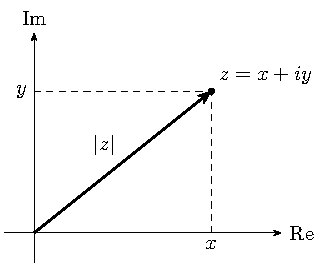
\includegraphics{figuras/plano-complejo.pdf}
    \caption{El número complejo $z=x+iy$ como vector.}
  \end{figure}

  Si $z_1=a_1+ib_1$ y $z_2=a_2+ib_2$, entonces $z_1+z_2=(a_1+a_2)+i(b_1+b_2)$, que corresponde a la suma de vectores (regla del paralelogramo).

  \begin{figure}[H]
    \centering
    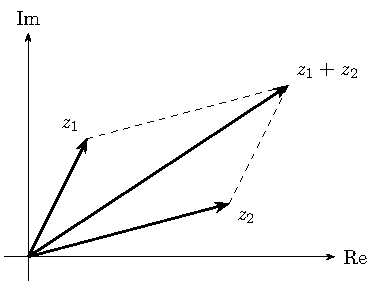
\includegraphics{figuras/suma-vectores.pdf}
    \caption{Suma de números complejos.}
  \end{figure}

  La distancia entre los puntos $z_1$ y $z_2$ es la longitud del vector $z_1-z_2$:
  \begin{equation*}
    |z_1-z_2|=\sqrt{(a_1-a_2)^2+(b_1-b_2)^2}.
  \end{equation*}

  Del módulo de $z=a+ib$ se sigue que $|z|^2=\Real^2\{z\}+\Imag^2\{z\}$, y de ahí la siguiente desigualdad.

  \begin{proposicion}\label{prop:re-im-modulo}
    Para todo $z\in\mathbb{C}$ se cumple
    \begin{equation*}
      \Real\{z\}\leq|\Real\{z\}|\leq|z|, \qquad \Imag\{z\}\leq|\Imag\{z\}|\leq|z|.
    \end{equation*}
  \end{proposicion}

  \begin{proof}
    Sea $z=a+ib$. La primera desigualdad de cada cadena es $a\leq|a|$ y $b\leq|b|$, válidas para todo real. Para la segunda, $|a|=\sqrt{a^2}\leq\sqrt{a^2+b^2}=|z|$, y análogamente $|b|=\sqrt{b^2}\leq\sqrt{a^2+b^2}=|z|$.
  \end{proof}

  % ======================================================
  \section{Desigualdad triangular}
  % ======================================================

  \begin{teorema}[Desigualdad triangular]
    Para todos $z_1,z_2\in\mathbb{C}$,
    \begin{equation*}
      |z_1+z_2|\leq|z_1|+|z_2|.
    \end{equation*}
  \end{teorema}

  \begin{proof}
    Usando $|w|^2=w\overline{w}$ con $w=z_1+z_2$ y las propiedades del conjugado,
    \begin{align*}
      |z_1+z_2|^2 & = (z_1+z_2)\,\overline{(z_1+z_2)}                                                                     \\
                  & = (z_1+z_2)(\overline{z_1}+\overline{z_2})                                                            \\
                  & = z_1\overline{z_1}+z_1\overline{z_2}+z_2\overline{z_1}+z_2\overline{z_2}                             \\
                  & = |z_1|^2+z_1\overline{z_2}+\overline{\left(z_1\overline{z_2}\right)}+|z_2|^2                          \\
                  & = |z_1|^2+2\Real\{z_1\overline{z_2}\}+|z_2|^2,
    \end{align*}
    donde en la cuarta línea usamos que $\overline{z_1\overline{z_2}}=\overline{z_1}\,\overline{\overline{z_2}}=\overline{z_1}\,z_2=z_2\overline{z_1}$, y en la quinta que $w+\overline{w}=2\Real\{w\}$.

    Por la proposición~\ref{prop:re-im-modulo}, aplicada a $w=z_1\overline{z_2}$, y por las propiedades del módulo,
    \begin{equation*}
      \Real\{z_1\overline{z_2}\}\leq|\Real\{z_1\overline{z_2}\}|\leq|z_1\overline{z_2}|=|z_1|\,|\overline{z_2}|=|z_1|\,|z_2|.
    \end{equation*}
    Multiplicando por $2$ y sumando $|z_1|^2+|z_2|^2$ en ambos lados,
    \begin{equation*}
      |z_1+z_2|^2\leq|z_1|^2+2|z_1||z_2|+|z_2|^2=\big(|z_1|+|z_2|\big)^2.
    \end{equation*}
    Como $|z_1+z_2|\geq 0$ y $|z_1|+|z_2|\geq 0$, al extraer raíz cuadrada se obtiene $|z_1+z_2|\leq|z_1|+|z_2|$.
  \end{proof}

  % ======================================================
  \section{Forma polar y argumento}
  % ======================================================

  Sea $z=x+iy\neq 0$. Además de las coordenadas rectangulares $(x,y)$, podemos describir al punto $z$ mediante su distancia $r$ al origen y el ángulo $\theta$ que forma el vector con el eje real positivo (medido en sentido antihorario), es decir, mediante las \textbf{coordenadas polares} $z=(r,\theta)$. De la figura,
  \begin{equation*}
    x=r\cos\theta, \qquad y=r\sin\theta, \qquad\text{y por lo tanto}\qquad z=r\cos\theta+ir\sin\theta=r(\cos\theta+i\sin\theta).
  \end{equation*}

  \begin{figure}[H]
    \centering
    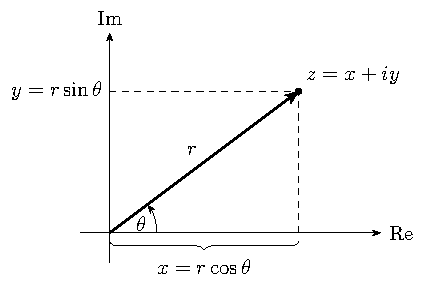
\includegraphics{figuras/forma-polar.pdf}
    \caption{Coordenadas polares de $z=x+iy$.}
  \end{figure}

  Si $r\geq 0$, entonces $r=|z|$. En efecto,
  \begin{align*}
    |z|^2=z\overline{z} & = r(\cos\theta+i\sin\theta)\,r(\cos\theta-i\sin\theta) \\
                        & = r^2\big[\cos^2\theta-i^2\sin^2\theta\big]            \\
                        & = r^2\big[\cos^2\theta+\sin^2\theta\big]=r^2,
  \end{align*}
  y como $r,|z|\geq 0$, resulta $r=|z|$. Así,
  \begin{equation*}
    z=|z|(\cos\theta+i\sin\theta).
  \end{equation*}
  Para encontrar el ángulo $\theta$ usamos que $\tan\theta=\dfrac{y}{x}$ (si $x\neq 0$); como la tangente sólo determina $\theta$ salvo múltiplos de $\pi$, hay que atender además al cuadrante en el que se encuentra $z$.

  \begin{definicion}[Argumento]
    Cada valor de $\theta$ tal que $z=|z|(\cos\theta+i\sin\theta)$ se denomina un \textbf{argumento} de $z$, y el conjunto de todos los argumentos se representa por $\arg(z)$. El \textbf{argumento principal} de $z$, denotado por $\Arg(z)$, es el argumento que cumple
    \begin{equation*}
      -\pi<\Arg(z)\leq\pi.
    \end{equation*}
  \end{definicion}

  Como $(r,\theta)$ y $(r,\theta+2\pi n)$ representan el mismo punto para todo $n\in\mathbb{Z}$, se cumple que
  \begin{equation*}
    \arg(z)=\{\Arg(z)+2n\pi : n\in\mathbb{Z}\}.
  \end{equation*}

  \begin{ejemplo}
    \textbf{Cálculo de $\Arg(w)$ y $\arg(w)$ para $w=-1-i$.} El punto $w$ está en el tercer cuadrante.

    \begin{figure}[H]
      \centering
      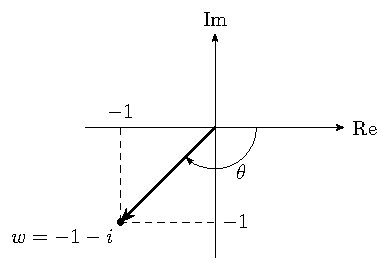
\includegraphics{figuras/argumento-w.pdf}
    \end{figure}

    Tenemos $\arctan\!\left(\dfrac{-1}{-1}\right)=\arctan(1)=\dfrac{\pi}{4}$, pero éste no es un argumento de $w$ (corresponde al primer cuadrante). Un argumento de $w$ es $\dfrac{\pi}{4}-\pi=-\dfrac{3\pi}{4}$, que está en $(-\pi,\pi]$. Como $|w|=\sqrt{2}$, se verifica $\sqrt{2}\cos(-\tfrac{3\pi}{4})=-1$ y $\sqrt{2}\sin(-\tfrac{3\pi}{4})=-1$. Por lo tanto
    \begin{align*}
      \Arg(w) & =-\frac{3\pi}{4},                                                                                                              \\
      \arg(w) & =\Big\{-\frac{3\pi}{4}+2n\pi : n\in\mathbb{Z}\Big\}=\Big\{\frac{(8n-3)\pi}{4} : n\in\mathbb{Z}\Big\}                         \\
              & =\Big\{\dots,-\frac{19\pi}{4},-\frac{11\pi}{4},-\frac{3\pi}{4},\frac{5\pi}{4},\frac{13\pi}{4},\dots\Big\}.
    \end{align*}
  \end{ejemplo}

  % ======================================================
  \section{Fórmula de Euler}
  % ======================================================

  Recordemos las series de potencias que definen a la exponencial, el seno y el coseno; convergen absolutamente para todo $z\in\mathbb{C}$:
  \begin{equation*}
    e^z=\sum_{n=0}^{\infty}\frac{z^n}{n!}, \qquad \sin(z)=\sum_{n=0}^{\infty}\frac{(-1)^nz^{2n+1}}{(2n+1)!}, \qquad \cos(z)=\sum_{n=0}^{\infty}\frac{(-1)^nz^{2n}}{(2n)!}.
  \end{equation*}
  Necesitaremos las potencias de $i$. Como $i^2=-1$, para todo entero $k\geq 0$,
  \begin{align*}
    i^{2k}   & =(i^2)^k=(-1)^k,          \\
    i^{2k+1} & =i^{2k}\cdot i=(-1)^k\,i.
  \end{align*}

  \begin{teorema}[Fórmula de Euler]
    Para todo $\theta\in\mathbb{R}$,
    \begin{equation*}
      e^{i\theta}=\cos\theta+i\sin\theta.
    \end{equation*}
  \end{teorema}

  \begin{proof}
    Sustituyendo $z=i\theta$ en la serie de la exponencial,
    \begin{equation*}
      e^{i\theta}=\sum_{n=0}^{\infty}\frac{(i\theta)^n}{n!}=\sum_{n=0}^{\infty}\frac{i^n\theta^n}{n!}=1+\frac{i\theta}{1!}+\frac{(i\theta)^2}{2!}+\frac{(i\theta)^3}{3!}+\frac{(i\theta)^4}{4!}+\cdots
    \end{equation*}
    Como la serie converge absolutamente, podemos separar los términos con $n$ par ($n=2k$) y con $n$ impar ($n=2k+1$):
    \begin{align*}
      e^{i\theta} & =\sum_{k=0}^{\infty}\frac{i^{2k}\theta^{2k}}{(2k)!}+\sum_{k=0}^{\infty}\frac{i^{2k+1}\theta^{2k+1}}{(2k+1)!} \\
                  & =\sum_{k=0}^{\infty}\frac{(-1)^k\theta^{2k}}{(2k)!}+i\sum_{k=0}^{\infty}\frac{(-1)^k\theta^{2k+1}}{(2k+1)!}    \\
                  & =\cos\theta+i\sin\theta.
    \end{align*}
  \end{proof}

  \textbf{Observación.} Evaluando las series de $\sin$ y $\cos$ en $z=i\theta$ y usando $(i\theta)^{2n+1}=(-1)^n\,i\,\theta^{2n+1}$ y $(i\theta)^{2n}=(-1)^n\theta^{2n}$ se obtiene
  \begin{equation*}
    \sin(i\theta)=i\sum_{n=0}^{\infty}\frac{\theta^{2n+1}}{(2n+1)!}, \qquad \cos(i\theta)=\sum_{n=0}^{\infty}\frac{\theta^{2n}}{(2n)!},
  \end{equation*}
  que no coinciden con $\sin\theta$ ni con $\cos\theta$. La fórmula de Euler surge de sustituir $z=i\theta$ en la serie de la exponencial, no en las del seno y el coseno.

  % ======================================================
  \section{Forma exponencial y operaciones}
  % ======================================================

  Sea $z=a+ib$ con $|z|=R$ y sea $\theta$ un argumento de $z$. Entonces $a=|z|\cos\theta$ y $b=|z|\sin\theta$, y por la fórmula de Euler
  \begin{equation*}
    z=|z|\cos\theta+i|z|\sin\theta=|z|(\cos\theta+i\sin\theta)=|z|e^{i\theta}.
  \end{equation*}
  Ésta es la \textbf{forma exponencial} de $z$: escribimos $z=Re^{i\theta}$ con $R=|z|$.

  Para operar en forma exponencial usaremos la propiedad $e^{u+v}=e^ue^v$ de la exponencial (válida para $u,v\in\mathbb{C}$; se sigue de la serie), en particular $e^{i\alpha}e^{i\beta}=e^{i(\alpha+\beta)}$ y $e^{i\theta}e^{-i\theta}=e^0=1$. Sean $z_1=r_1e^{i\theta_1}$ y $z_2=r_2e^{i\theta_2}$ dos números complejos no nulos.

  \begin{itemize}
    \item \textbf{Producto:}
          \begin{equation*}
            z_1z_2=r_1e^{i\theta_1}\,r_2e^{i\theta_2}=r_1r_2\,e^{i(\theta_1+\theta_2)}.
          \end{equation*}
    \item \textbf{Inverso:} $z_2^{-1}=\dfrac{1}{r_2}e^{-i\theta_2}$, pues $\big(r_2e^{i\theta_2}\big)\big(\tfrac{1}{r_2}e^{-i\theta_2}\big)=e^{i\theta_2}e^{-i\theta_2}=1$.
    \item \textbf{División:}
          \begin{equation*}
            \frac{z_1}{z_2}=z_1z_2^{-1}=\frac{r_1e^{i\theta_1}}{r_2e^{i\theta_2}}=\frac{r_1}{r_2}\,e^{i(\theta_1-\theta_2)}.
          \end{equation*}
    \item \textbf{Potencia:} si $z=re^{i\theta}\neq 0$ y $n\in\mathbb{Z}$, entonces
          \begin{equation*}
            z^n=r^ne^{in\theta}.
          \end{equation*}
  \end{itemize}

  \begin{proof}[Demostración de la fórmula de la potencia]
    Primero probamos, por inducción sobre $n$, el caso $n\geq 0$.

    \textbf{Base inductiva.} Para $n=0$, $z^0=1=r^0e^{0}$; para $n=1$, $z^1=re^{i\theta}$; y para $n=2$, $z^2=zz=re^{i\theta}\,re^{i\theta}=r^2e^{i2\theta}$.

    \textbf{Hipótesis inductiva.} $z^k=r^ke^{ik\theta}$ para algún $k\geq 0$.

    \textbf{Paso inductivo.}
    \begin{equation*}
      z^{k+1}=z^kz=r^ke^{ik\theta}\,re^{i\theta}=r^{k+1}e^{i(k\theta+\theta)}=r^{k+1}e^{i(k+1)\theta}.
    \end{equation*}
    Para $n<0$, escribimos $n=-m$ con $m>0$. Como $z^{-1}=\frac{1}{r}e^{i(-\theta)}$, el caso ya probado aplicado a $z^{-1}$ da
    \begin{equation*}
      z^n=(z^{-1})^m=\Big(\frac{1}{r}\Big)^m e^{i(-\theta)m}=r^{-m}e^{-im\theta}=r^ne^{in\theta}.\qedhere
    \end{equation*}
  \end{proof}

  % ======================================================
  \section{Fórmula de De Moivre}
  % ======================================================

  Si en la fórmula de la potencia tomamos $r=1$, entonces $z=e^{i\theta}$ y $z^n=e^{in\theta}$, es decir, $e^{in\theta}=(e^{i\theta})^n$. Aplicando la fórmula de Euler a ambos lados obtenemos:

  \begin{teorema}[Fórmula de De Moivre]
    Para todo $\theta\in\mathbb{R}$ y todo $n\in\mathbb{Z}$,
    \begin{equation*}
      (\cos\theta+i\sin\theta)^n=\cos(n\theta)+i\sin(n\theta).
    \end{equation*}
  \end{teorema}

  \begin{ejercicio}
    Expresar $\cos(2\theta)$ y $\sin(2\theta)$ en términos de $\cos\theta$ y $\sin\theta$.
  \end{ejercicio}

  \begin{solucion}
    Por la fórmula de Euler y el desarrollo del cuadrado,
    \begin{equation*}
      e^{i2\theta}=(e^{i\theta})^2=(\cos\theta+i\sin\theta)^2=\cos^2\theta+2i\cos\theta\sin\theta-\sin^2\theta.
    \end{equation*}
    Por otro lado, $e^{i2\theta}=\cos(2\theta)+i\sin(2\theta)$. Igualando partes real e imaginaria,
    \begin{equation*}
      \cos(2\theta)=\cos^2\theta-\sin^2\theta, \qquad \sin(2\theta)=2\cos\theta\sin\theta.
    \end{equation*}
  \end{solucion}

  \begin{ejercicio}
    Encontrar una expresión para $\cos(\alpha+\beta)$ y $\sin(\alpha+\beta)$.
  \end{ejercicio}

  \begin{solucion}
    Por un lado, $e^{i\alpha}e^{i\beta}=e^{i(\alpha+\beta)}=\cos(\alpha+\beta)+i\sin(\alpha+\beta)$. Por otro,
    \begin{align*}
      e^{i\alpha}e^{i\beta} & =(\cos\alpha+i\sin\alpha)(\cos\beta+i\sin\beta)                                                         \\
                            & =\cos\alpha\cos\beta+i\cos\alpha\sin\beta+i\sin\alpha\cos\beta-\sin\alpha\sin\beta                      \\
                            & =\big[\cos\alpha\cos\beta-\sin\alpha\sin\beta\big]+i\big[\cos\alpha\sin\beta+\sin\alpha\cos\beta\big].
    \end{align*}
    Igualando partes real e imaginaria,
    \begin{align*}
      \cos(\alpha+\beta) & =\cos\alpha\cos\beta-\sin\alpha\sin\beta, \\
      \sin(\alpha+\beta) & =\cos\alpha\sin\beta+\sin\alpha\cos\beta.
    \end{align*}
  \end{solucion}

  Para obtener expresiones de $\cos(n\theta)$ y $\sin(n\theta)$ para un $n\in\mathbb{N}$ cualquiera, combinamos la fórmula de De Moivre con el teorema del binomio.

  \begin{teorema}[Teorema del binomio]
    Para $a,b\in\mathbb{C}$ y $n\in\mathbb{N}$,
    \begin{equation*}
      (a+b)^n=\sum_{k=0}^{n}\binom{n}{k}a^{n-k}b^k, \qquad \binom{n}{k}=\frac{n!}{k!\,(n-k)!}.
    \end{equation*}
  \end{teorema}

  Separando los sumandos con $k$ par ($k=2k'$) y con $k$ impar ($k=2k'+1$), y escribiendo de nuevo $k$ en vez de $k'$:
  \begin{equation*}
    (a+b)^n=\sum_{k=0}^{\lfloor n/2\rfloor}\binom{n}{2k}a^{n-2k}b^{2k}+\sum_{k=0}^{\lfloor (n-1)/2\rfloor}\binom{n}{2k+1}a^{n-2k-1}b^{2k+1}.
  \end{equation*}
  Tomemos $a=\cos\theta$ y $b=i\sin\theta$. Como $b^{2k}=i^{2k}\sin^{2k}\theta=(-1)^k\sin^{2k}\theta$ y $b^{2k+1}=(-1)^k\,i\,\sin^{2k+1}\theta$,
  \begin{equation*}
    (\cos\theta+i\sin\theta)^n=\sum_{k=0}^{\lfloor n/2\rfloor}(-1)^k\binom{n}{2k}\cos^{n-2k}\theta\sin^{2k}\theta+i\sum_{k=0}^{\lfloor (n-1)/2\rfloor}(-1)^k\binom{n}{2k+1}\cos^{n-2k-1}\theta\sin^{2k+1}\theta.
  \end{equation*}
  Ambas sumas son reales, así que, comparando con la fórmula de De Moivre, obtenemos:
  \begin{align*}
    \cos(n\theta) & =\sum_{k=0}^{\lfloor n/2\rfloor}(-1)^k\binom{n}{2k}\cos^{n-2k}\theta\sin^{2k}\theta,         \\
    \sin(n\theta) & =\sum_{k=0}^{\lfloor (n-1)/2\rfloor}(-1)^k\binom{n}{2k+1}\cos^{n-2k-1}\theta\sin^{2k+1}\theta.
  \end{align*}
  Por ejemplo, para $n=3$: $\cos(3\theta)=\cos^3\theta-3\cos\theta\sin^2\theta$ y $\sin(3\theta)=3\cos^2\theta\sin\theta-\sin^3\theta$.

  % ======================================================
  \section{Raíces de números complejos}
  % ======================================================

  Sean $z_1=r_1e^{i\theta_1}$ y $z_2=r_2e^{i\theta_2}$ dos números complejos no nulos (con $r_1,r_2>0$). Entonces
  \begin{equation*}
    z_1=z_2 \iff r_1=r_2 \ \text{ y } \ \theta_1=\theta_2+2k\pi \text{ para algún } k\in\mathbb{Z}.
  \end{equation*}
  En efecto, si $z_1=z_2$, al tomar módulos $r_1=r_2$; dividiendo entre $r_1$ queda $e^{i\theta_1}=e^{i\theta_2}$, es decir, $\cos\theta_1=\cos\theta_2$ y $\sin\theta_1=\sin\theta_2$, lo que ocurre si y sólo si $\theta_1-\theta_2$ es un múltiplo entero de $2\pi$. El recíproco es inmediato.

  \begin{definicion}[Raíz $n$-ésima]
    Sean $n\in\mathbb{N}$ y $z_0\in\mathbb{C}$. Un número $z\in\mathbb{C}$ es una \textbf{raíz $n$-ésima} de $z_0$ si $z^n=z_0$; es decir, $z$ multiplicado por sí mismo $n$ veces da $z_0$.
  \end{definicion}

  \begin{teorema}[Raíces $n$-ésimas]
    Sea $z_0=r_0e^{i\theta_0}\neq 0$ y $n\in\mathbb{N}$. La ecuación $z^n=z_0$ tiene exactamente $n$ soluciones distintas, dadas por
    \begin{equation*}
      w_k=r_0^{1/n}\,e^{i\left(\frac{\theta_0}{n}+\frac{2\pi k}{n}\right)}, \qquad k=0,1,\dots,n-1.
    \end{equation*}
  \end{teorema}

  \begin{proof}
    Como $z_0\neq 0$, toda solución es no nula; escribamos $z=re^{i\theta}$ con $r>0$. Entonces $z^n=z_0$ equivale a $r^ne^{in\theta}=r_0e^{i\theta_0}$, y por el criterio de igualdad,
    \begin{equation*}
      r^n=r_0 \quad\text{y}\quad n\theta=\theta_0+2\pi k\ \text{ para algún } k\in\mathbb{Z}.
    \end{equation*}
    La primera condición da $r=\sqrt[n]{r_0}=r_0^{1/n}$ (la única raíz positiva), y la segunda da $\theta=\dfrac{\theta_0}{n}+\dfrac{2\pi k}{n}$. Así, toda solución es de la forma $w_k$ con $k\in\mathbb{Z}$, y recíprocamente cada $w_k$ es solución.

    Falta ver cuáles de ellas son distintas. Por el criterio de igualdad, $w_k=w_{k'}$ si y sólo si $\dfrac{2\pi(k-k')}{n}$ es múltiplo entero de $2\pi$, es decir, si y sólo si $n\mid k-k'$. Por lo tanto, cada $k\in\mathbb{Z}$ da la misma raíz que un único $k\in\{0,\dots,n-1\}$, y estas $n$ raíces son distintas entre sí.
  \end{proof}

  Geométricamente, las $n$ raíces están sobre la circunferencia de radio $r_0^{1/n}$ centrada en el origen, y son los vértices de un polígono regular de $n$ lados.

  \begin{ejemplo}
    \textbf{Raíces cúbicas de $z_0=3+3i$.} Calculamos
    \begin{equation*}
      r_0=\sqrt{3^2+3^2}=\sqrt{2\cdot 9}=3\sqrt{2}, \qquad \theta_0=\arctan\!\Big(\frac{3}{3}\Big)=\arctan(1)=\frac{\pi}{4},
    \end{equation*}
    (el punto está en el primer cuadrante), de modo que $z_0=3\sqrt{2}\,e^{i\pi/4}$. Para $n=3$,
    \begin{equation*}
      r=\sqrt[3]{3\sqrt{2}}=3^{1/3}2^{1/6}, \qquad \theta=\frac{\theta_0}{n}+\frac{2k\pi}{n}=\frac{\pi}{4\cdot 3}+\frac{2k\pi}{3}=\frac{\pi}{12}+\frac{2k}{3}\pi.
    \end{equation*}
    Con $r=3^{1/3}2^{1/6}$, las tres raíces son
    \begin{align*}
      w_0 & =r\,e^{i\pi/12},                                                    \\
      w_1 & =r\,e^{i\left(\frac{\pi}{12}+\frac{2\pi}{3}\right)}=r\,e^{i3\pi/4},  \\
      w_2 & =r\,e^{i\left(\frac{\pi}{12}+\frac{4\pi}{3}\right)}=r\,e^{i17\pi/12}.
    \end{align*}
    Están sobre la circunferencia $|z|=r$ y forman un triángulo equilátero.

    \begin{figure}[H]
      \centering
      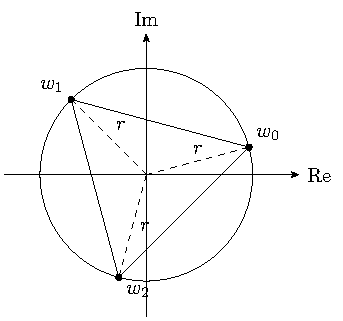
\includegraphics{figuras/raices-cubicas.pdf}
    \end{figure}
  \end{ejemplo}

  \subsection*{Resumen del capítulo}
  
  A lo largo de este capítulo construimos $\mathbb{R}$ a partir de tres tipos de axiomas: los \textbf{axiomas de cuerpo} (que rigen la suma y el producto), los \textbf{axiomas de orden} (que nos permiten comparar números), y el \textbf{axioma de completitud} (que garantiza la existencia de supremos e ínfimos, y es lo que distingue a $\mathbb{R}$ de $\mathbb{Q}$). A partir de ahí, usando la noción de conjunto inductivo, definimos a los enteros $\mathbb{Z}$ y estudiamos el principio de inducción matemática, una de las herramientas de demostración más importantes del curso. Terminamos con divisibilidad y números primos: el máximo común divisor, el lema y el primer teorema de Euclides, la infinitud de los primos, los primos de Mersenne y de Fermat, y el teorema fundamental de la aritmética. Por último, extendimos $\mathbb{R}$ al sistema $\mathbb{C}$ de los números complejos: los definimos como pares ordenados de reales y estudiamos su álgebra, el conjugado y el módulo, la desigualdad triangular, la forma polar y exponencial (fórmula de Euler), la fórmula de De Moivre y las raíces $n$-ésimas. Todas estas ideas —los axiomas de $\mathbb{R}$, la inducción, y la aritmética de los enteros— reaparecerán constantemente en el resto del curso.

  % ======================================================
  \chapter{Teoría de conjuntos}
  % ======================================================

  En este capítulo ampliamos el lenguaje básico de conjuntos de la sección 1.1 y formalizamos las nociones de par ordenado, producto cartesiano, relación y función.

  % ======================================================
  \section{Pares ordenados y producto cartesiano}
  % ======================================================

  Un conjunto no distingue el orden de sus elementos: $\{a,b\}=\{b,a\}$. Para poder hablar de un ``primer'' y un ``segundo'' elemento necesitamos un objeto nuevo.

  \begin{definicion}[Par ordenado]
    Dados dos objetos $a$ y $b$, el \textbf{par ordenado} $(a,b)$ es el conjunto
    \begin{equation*}
      (a,b)=\big\{\{a\},\{a,b\}\big\}.
    \end{equation*}
  \end{definicion}

  Los elementos de $(a,b)$ son los conjuntos $\{a\}$ y $\{a,b\}$ (que coinciden cuando $a=b$). Por ejemplo,
  \begin{equation*}
    (a,b)=\big\{\{a\},\{a,b\}\big\}, \qquad (b,a)=\big\{\{b\},\{a,b\}\big\}.
  \end{equation*}
  El siguiente teorema muestra que esta definición captura justamente lo que esperamos de un par ordenado.

  \begin{teorema}[Igualdad de pares ordenados]\label{teo:igualdad-pares}
    $(a,b)=(c,d)$ si y sólo si $a=c$ y $b=d$.
  \end{teorema}

  \begin{proof}
    ($\Leftarrow$) Si $a=c$ y $b=d$, los conjuntos $(a,b)$ y $(c,d)$ son literalmente el mismo.

    ($\Rightarrow$) Supongamos que $\big\{\{a\},\{a,b\}\big\}=\big\{\{c\},\{c,d\}\big\}$ y distingamos dos casos.

    \textit{Caso 1: $a=b$.} Entonces $\{a\}=\{a,b\}$, así que el conjunto de la izquierda es $\{\{a\}\}$ y tiene un único elemento. Por lo tanto $\{c\}=\{a\}$ y $\{c,d\}=\{a\}$. De la primera igualdad, $c=a$; de la segunda, $d=a$. Así, $a=c$ y $b=a=d$.

    \textit{Caso 2: $a\neq b$.} Entonces $\{a\}\neq\{a,b\}$ (pues $b\in\{a,b\}$ pero $b\notin\{a\}$), de modo que el conjunto de la izquierda tiene dos elementos. Como $\{a\}$ pertenece al conjunto de la izquierda, también pertenece al de la derecha: $\{a\}=\{c\}$ o $\{a\}=\{c,d\}$. Si fuera $\{a\}=\{c,d\}$, tendríamos $c=d=a$ y el conjunto de la derecha sería $\{\{a\}\}$, con un solo elemento, lo cual es imposible. Luego $\{a\}=\{c\}$, es decir, $a=c$. Ahora bien, $\{a,b\}$ pertenece al conjunto de la derecha y $\{a,b\}\neq\{a\}=\{c\}$, así que $\{a,b\}=\{c,d\}=\{a,d\}$. Como $b\in\{a,d\}$ y $b\neq a$, concluimos que $b=d$.
  \end{proof}

  En particular, $(a,b)=(b,a)$ si y sólo si $a=b$; es decir, en general $(a,b)\neq(b,a)$.

  \begin{definicion}[Producto cartesiano]
    Dados dos conjuntos $A$ y $B$, el \textbf{producto cartesiano} de $A$ y $B$, denotado por $A\times B$, es el conjunto de todos los pares ordenados $(a,b)$ tales que $a\in A$ y $b\in B$:
    \begin{equation*}
      A\times B=\{(a,b) : a\in A \text{ y } b\in B\}.
    \end{equation*}
  \end{definicion}

  Los elementos de $A\times B$ son los pares $(a,b)$, y no los elementos $a$ y $b$ por separado.

  \begin{ejemplo}
    $\mathbb{R}^2=\mathbb{R}\times\mathbb{R}$ y $\mathbb{R}^3=\mathbb{R}\times\mathbb{R}\times\mathbb{R}$. Notemos que $\mathbb{R}^2\not\subset\mathbb{R}^3$: los elementos de $\mathbb{R}^2$ son pares y los de $\mathbb{R}^3$ son ternas.
  \end{ejemplo}

  % ======================================================
  \section{Relaciones y funciones}
  % ======================================================

  Sean $x,y\in\mathbb{R}$. Identificamos el par ordenado $(x,y)\in\mathbb{R}\times\mathbb{R}$ con el punto del plano cuyas coordenadas rectangulares son $x$ y $y$. Con esta identificación, condiciones como $x^2+y^2\leq 1$ o $x^2+y^2=1$ determinan subconjuntos del plano:
  \begin{align*}
    S_1 & = \{(x,y) : x^2+y^2\leq 1\}, \\
    S_2 & = \{(x,y) : x^2+y^2=1\},
  \end{align*}
  y se cumple que $S_1\subset\mathbb{R}\times\mathbb{R}$ y $S_2\subset\mathbb{R}\times\mathbb{R}$.

  \begin{figure}[H]
    \centering
    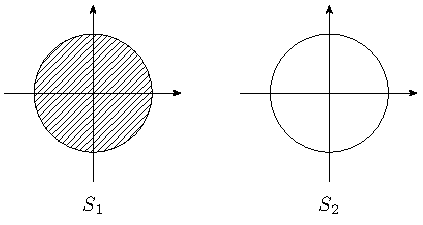
\includegraphics{figuras/relaciones-disco-circulo.pdf}
    \caption{El disco $S_1$ y la circunferencia $S_2$.}
  \end{figure}

  \begin{definicion}[Relación]
    Se llama \textbf{relación} a todo conjunto de pares ordenados.
  \end{definicion}

  Sea $S=\{(a_1,b_1),(a_2,b_2),(a_3,b_3),\dots\}$ una relación. El conjunto formado por todos los primeros elementos de los pares de $S$ se denomina el \textbf{dominio} de $S$ y se representa por
  \begin{equation*}
    \operatorname{dom}S=\{a_1,a_2,a_3,\dots\}.
  \end{equation*}
  El conjunto formado por todos los segundos elementos de los pares de $S$ se llama \textbf{recorrido} de $S$ (también, en estas notas, \textbf{contradominio} o \textbf{codominio}; en otros textos, el codominio es cualquier conjunto que contiene al recorrido).

  \begin{definicion}[Gráfica de una relación]
    La \textbf{gráfica} de una relación es el conjunto de puntos del plano que corresponden a los pares ordenados de la relación.
  \end{definicion}

  Por ejemplo, el par $(2,3)$ corresponde al punto del plano de abscisa $2$ y ordenada $3$.

  \begin{definicion}[Función]
    Una \textbf{función} $F$ es un conjunto de pares ordenados $(x,y)$ ninguno de los cuales tiene el mismo primer elemento que otro. Es decir, si $(x,y)\in F$ y $(x,z)\in F$, entonces $y=z$.
  \end{definicion}

  En otras palabras, una función es una relación en la que cada elemento del dominio aparece como primer elemento de exactamente un par. Geométricamente, la gráfica de una relación es la de una función si y sólo si toda recta vertical la interseca a lo más en un punto.

  \begin{ejemplo}
    La circunferencia $S_2$ no es una función: $(0,1)\in S_2$ y $(0,-1)\in S_2$ tienen el mismo primer elemento, pero $1\neq -1$. Lo mismo ocurre con el disco $S_1$. En cambio, $F=\{(x,x^3) : x\in\mathbb{R}\}$ sí es una función: si $(x,y)\in F$ y $(x,z)\in F$, entonces $y=x^3=z$.
  \end{ejemplo}

  \begin{figure}[H]
    \centering
    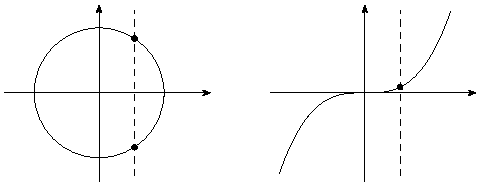
\includegraphics{figuras/recta-vertical.pdf}
    \caption{Una relación que no es función (izquierda) y una que sí lo es (derecha).}
  \end{figure}

\end{document}